\documentclass[11pt]{article}
\renewcommand{\arraystretch}{1.5} % Default value: 1
\usepackage{sectsty}
\allsectionsfont{\color{blue}\fontfamily{lmss}\selectfont}
\usepackage{fontspec}
\setmainfont{XCharter}

\usepackage{listings}

\lstset{
basicstyle=\small\ttfamily,
tabsize=8,
columns=flexible,
breaklines=true,
frame=tb,
rulecolor=\color[rgb]{0.8,0.8,0.7},
backgroundcolor=\color[rgb]{1,1,0.91},
postbreak=\raisebox{0ex}[0ex][0ex]{\ensuremath{\color{red}\hookrightarrow\space}}
}
\usepackage{fontawesome}


\usepackage{mdframed}
\newmdenv[
  backgroundcolor=gray,
  fontcolor=white,
  nobreak=true,
]{terminalinput}



\usepackage{parskip}


    \usepackage[breakable]{tcolorbox}
    \usepackage{parskip} % Stop auto-indenting (to mimic markdown behaviour)

    \usepackage{iftex}
    \ifPDFTeX
    	\usepackage[T1]{fontenc}
    	\usepackage{mathpazo}
    \else
    	\usepackage{fontspec}
    \fi

    % Basic figure setup, for now with no caption control since it's done
    % automatically by Pandoc (which extracts ![](path) syntax from Markdown).
    \usepackage{graphicx}
    % Maintain compatibility with old templates. Remove in nbconvert 6.0
    \let\Oldincludegraphics\includegraphics
    % Ensure that by default, figures have no caption (until we provide a
    % proper Figure object with a Caption API and a way to capture that
    % in the conversion process - todo).
    \usepackage{caption}
    \DeclareCaptionFormat{nocaption}{}
    \captionsetup{labelformat=nolabel, textfont=bf}

    \usepackage{float}
    \floatplacement{figure}{H} % forces figures to be placed at the correct location
    \usepackage{xcolor} % Allow colors to be defined
    \usepackage{enumerate} % Needed for markdown enumerations to work
    \usepackage{geometry} % Used to adjust the document margins
    \usepackage{amsmath} % Equations
    \usepackage{amssymb} % Equations
    \usepackage{textcomp} % defines textquotesingle
    % Hack from http://tex.stackexchange.com/a/47451/13684:
    \AtBeginDocument{%
        \def\PYZsq{\textquotesingle}% Upright quotes in Pygmentized code
    }
    \usepackage{upquote} % Upright quotes for verbatim code
    \usepackage{eurosym} % defines \euro
    \usepackage[mathletters]{ucs} % Extended unicode (utf-8) support
    \usepackage{fancyvrb} % verbatim replacement that allows latex
    \usepackage{grffile} % extends the file name processing of package graphics
                         % to support a larger range
    \makeatletter % fix for old versions of grffile with XeLaTeX
    \@ifpackagelater{grffile}{2019/11/01}
    {
      % Do nothing on new versions
    }
    {
      \def\Gread@@xetex#1{%
        \IfFileExists{"\Gin@base".bb}%
        {\Gread@eps{\Gin@base.bb}}%
        {\Gread@@xetex@aux#1}%
      }
    }
    \makeatother
    \usepackage[Export]{adjustbox} % Used to constrain images to a maximum size
    \adjustboxset{max size={0.9\linewidth}{0.9\paperheight}}

    % The hyperref package gives us a pdf with properly built
    % internal navigation ('pdf bookmarks' for the table of contents,
    % internal cross-reference links, web links for URLs, etc.)
    \usepackage{hyperref}
    % The default LaTeX title has an obnoxious amount of whitespace. By default,
    % titling removes some of it. It also provides customization options.
    \usepackage{titling}
    \usepackage{longtable} % longtable support required by pandoc >1.10
    \usepackage{booktabs}  % table support for pandoc > 1.12.2
    \usepackage[inline]{enumitem} % IRkernel/repr support (it uses the enumerate* environment)
    \usepackage[normalem]{ulem} % ulem is needed to support strikethroughs (\sout)
                                % normalem makes italics be italics, not underlines
    \usepackage{mathrsfs}



    % Colors for the hyperref package
    \definecolor{urlcolor}{rgb}{0,.145,.698}
    \definecolor{linkcolor}{rgb}{.71,0.21,0.01}
    \definecolor{citecolor}{rgb}{.12,.54,.11}

    % ANSI colors
    \definecolor{ansi-black}{HTML}{3E424D}
    \definecolor{ansi-black-intense}{HTML}{282C36}
    \definecolor{ansi-red}{HTML}{E75C58}
    \definecolor{ansi-red-intense}{HTML}{B22B31}
    \definecolor{ansi-green}{HTML}{00A250}
    \definecolor{ansi-green-intense}{HTML}{007427}
    \definecolor{ansi-yellow}{HTML}{DDB62B}
    \definecolor{ansi-yellow-intense}{HTML}{B27D12}
    \definecolor{ansi-blue}{HTML}{208FFB}
    \definecolor{ansi-blue-intense}{HTML}{0065CA}
    \definecolor{ansi-magenta}{HTML}{D160C4}
    \definecolor{ansi-magenta-intense}{HTML}{A03196}
    \definecolor{ansi-cyan}{HTML}{60C6C8}
    \definecolor{ansi-cyan-intense}{HTML}{258F8F}
    \definecolor{ansi-white}{HTML}{C5C1B4}
    \definecolor{ansi-white-intense}{HTML}{A1A6B2}
    \definecolor{ansi-default-inverse-fg}{HTML}{FFFFFF}
    \definecolor{ansi-default-inverse-bg}{HTML}{000000}

    % common color for the border for error outputs.
    \definecolor{outerrorbackground}{HTML}{FFDFDF}

    % commands and environments needed by pandoc snippets
    % extracted from the output of `pandoc -s`
    \providecommand{\tightlist}{%
      \setlength{\itemsep}{0pt}\setlength{\parskip}{0pt}}
    \DefineVerbatimEnvironment{Highlighting}{Verbatim}{commandchars=\\\{\}}
    % Add ',fontsize=\small' for more characters per line
    \newenvironment{Shaded}{}{}
    \newcommand{\KeywordTok}[1]{\textcolor[rgb]{0.00,0.44,0.13}{\textbf{{#1}}}}
    \newcommand{\DataTypeTok}[1]{\textcolor[rgb]{0.56,0.13,0.00}{{#1}}}
    \newcommand{\DecValTok}[1]{\textcolor[rgb]{0.25,0.63,0.44}{{#1}}}
    \newcommand{\BaseNTok}[1]{\textcolor[rgb]{0.25,0.63,0.44}{{#1}}}
    \newcommand{\FloatTok}[1]{\textcolor[rgb]{0.25,0.63,0.44}{{#1}}}
    \newcommand{\CharTok}[1]{\textcolor[rgb]{0.25,0.44,0.63}{{#1}}}
    \newcommand{\StringTok}[1]{\textcolor[rgb]{0.25,0.44,0.63}{{#1}}}
    \newcommand{\CommentTok}[1]{\textcolor[rgb]{0.38,0.63,0.69}{\textit{{#1}}}}
    \newcommand{\OtherTok}[1]{\textcolor[rgb]{0.00,0.44,0.13}{{#1}}}
    \newcommand{\AlertTok}[1]{\textcolor[rgb]{1.00,0.00,0.00}{\textbf{{#1}}}}
    \newcommand{\FunctionTok}[1]{\textcolor[rgb]{0.02,0.16,0.49}{{#1}}}
    \newcommand{\RegionMarkerTok}[1]{{#1}}
    \newcommand{\ErrorTok}[1]{\textcolor[rgb]{1.00,0.00,0.00}{\textbf{{#1}}}}
    \newcommand{\NormalTok}[1]{{#1}}

    % Additional commands for more recent versions of Pandoc
    \newcommand{\ConstantTok}[1]{\textcolor[rgb]{0.53,0.00,0.00}{{#1}}}
    \newcommand{\SpecialCharTok}[1]{\textcolor[rgb]{0.25,0.44,0.63}{{#1}}}
    \newcommand{\VerbatimStringTok}[1]{\textcolor[rgb]{0.25,0.44,0.63}{{#1}}}
    \newcommand{\SpecialStringTok}[1]{\textcolor[rgb]{0.73,0.40,0.53}{{#1}}}
    \newcommand{\ImportTok}[1]{{#1}}
    \newcommand{\DocumentationTok}[1]{\textcolor[rgb]{0.73,0.13,0.13}{\textit{{#1}}}}
    \newcommand{\AnnotationTok}[1]{\textcolor[rgb]{0.38,0.63,0.69}{\textbf{\textit{{#1}}}}}
    \newcommand{\CommentVarTok}[1]{\textcolor[rgb]{0.38,0.63,0.69}{\textbf{\textit{{#1}}}}}
    \newcommand{\VariableTok}[1]{\textcolor[rgb]{0.10,0.09,0.49}{{#1}}}
    \newcommand{\ControlFlowTok}[1]{\textcolor[rgb]{0.00,0.44,0.13}{\textbf{{#1}}}}
    \newcommand{\OperatorTok}[1]{\textcolor[rgb]{0.40,0.40,0.40}{{#1}}}
    \newcommand{\BuiltInTok}[1]{{#1}}
    \newcommand{\ExtensionTok}[1]{{#1}}
    \newcommand{\PreprocessorTok}[1]{\textcolor[rgb]{0.74,0.48,0.00}{{#1}}}
    \newcommand{\AttributeTok}[1]{\textcolor[rgb]{0.49,0.56,0.16}{{#1}}}
    \newcommand{\InformationTok}[1]{\textcolor[rgb]{0.38,0.63,0.69}{\textbf{\textit{{#1}}}}}
    \newcommand{\WarningTok}[1]{\textcolor[rgb]{0.38,0.63,0.69}{\textbf{\textit{{#1}}}}}


    % Define a nice break command that doesn't care if a line doesn't already
    % exist.
    \def\br{\hspace*{\fill} \\* }
    % Math Jax compatibility definitions
    \def\gt{>}
    \def\lt{<}
    \let\Oldtex\TeX
    \let\Oldlatex\LaTeX
    \renewcommand{\TeX}{\textrm{\Oldtex}}
    \renewcommand{\LaTeX}{\textrm{\Oldlatex}}
    % Document parameters
    % Document title
    \title{index}





% Pygments definitions
\makeatletter
\def\PY@reset{\let\PY@it=\relax \let\PY@bf=\relax%
    \let\PY@ul=\relax \let\PY@tc=\relax%
    \let\PY@bc=\relax \let\PY@ff=\relax}
\def\PY@tok#1{\csname PY@tok@#1\endcsname}
\def\PY@toks#1+{\ifx\relax#1\empty\else%
    \PY@tok{#1}\expandafter\PY@toks\fi}
\def\PY@do#1{\PY@bc{\PY@tc{\PY@ul{%
    \PY@it{\PY@bf{\PY@ff{#1}}}}}}}
\def\PY#1#2{\PY@reset\PY@toks#1+\relax+\PY@do{#2}}

\expandafter\def\csname PY@tok@w\endcsname{\def\PY@tc##1{\textcolor[rgb]{0.73,0.73,0.73}{##1}}}
\expandafter\def\csname PY@tok@c\endcsname{\let\PY@it=\textit\def\PY@tc##1{\textcolor[rgb]{0.25,0.50,0.50}{##1}}}
\expandafter\def\csname PY@tok@cp\endcsname{\def\PY@tc##1{\textcolor[rgb]{0.74,0.48,0.00}{##1}}}
\expandafter\def\csname PY@tok@k\endcsname{\let\PY@bf=\textbf\def\PY@tc##1{\textcolor[rgb]{0.00,0.50,0.00}{##1}}}
\expandafter\def\csname PY@tok@kp\endcsname{\def\PY@tc##1{\textcolor[rgb]{0.00,0.50,0.00}{##1}}}
\expandafter\def\csname PY@tok@kt\endcsname{\def\PY@tc##1{\textcolor[rgb]{0.69,0.00,0.25}{##1}}}
\expandafter\def\csname PY@tok@o\endcsname{\def\PY@tc##1{\textcolor[rgb]{0.40,0.40,0.40}{##1}}}
\expandafter\def\csname PY@tok@ow\endcsname{\let\PY@bf=\textbf\def\PY@tc##1{\textcolor[rgb]{0.67,0.13,1.00}{##1}}}
\expandafter\def\csname PY@tok@nb\endcsname{\def\PY@tc##1{\textcolor[rgb]{0.00,0.50,0.00}{##1}}}
\expandafter\def\csname PY@tok@nf\endcsname{\def\PY@tc##1{\textcolor[rgb]{0.00,0.00,1.00}{##1}}}
\expandafter\def\csname PY@tok@nc\endcsname{\let\PY@bf=\textbf\def\PY@tc##1{\textcolor[rgb]{0.00,0.00,1.00}{##1}}}
\expandafter\def\csname PY@tok@nn\endcsname{\let\PY@bf=\textbf\def\PY@tc##1{\textcolor[rgb]{0.00,0.00,1.00}{##1}}}
\expandafter\def\csname PY@tok@ne\endcsname{\let\PY@bf=\textbf\def\PY@tc##1{\textcolor[rgb]{0.82,0.25,0.23}{##1}}}
\expandafter\def\csname PY@tok@nv\endcsname{\def\PY@tc##1{\textcolor[rgb]{0.10,0.09,0.49}{##1}}}
\expandafter\def\csname PY@tok@no\endcsname{\def\PY@tc##1{\textcolor[rgb]{0.53,0.00,0.00}{##1}}}
\expandafter\def\csname PY@tok@nl\endcsname{\def\PY@tc##1{\textcolor[rgb]{0.63,0.63,0.00}{##1}}}
\expandafter\def\csname PY@tok@ni\endcsname{\let\PY@bf=\textbf\def\PY@tc##1{\textcolor[rgb]{0.60,0.60,0.60}{##1}}}
\expandafter\def\csname PY@tok@na\endcsname{\def\PY@tc##1{\textcolor[rgb]{0.49,0.56,0.16}{##1}}}
\expandafter\def\csname PY@tok@nt\endcsname{\let\PY@bf=\textbf\def\PY@tc##1{\textcolor[rgb]{0.00,0.50,0.00}{##1}}}
\expandafter\def\csname PY@tok@nd\endcsname{\def\PY@tc##1{\textcolor[rgb]{0.67,0.13,1.00}{##1}}}
\expandafter\def\csname PY@tok@s\endcsname{\def\PY@tc##1{\textcolor[rgb]{0.73,0.13,0.13}{##1}}}
\expandafter\def\csname PY@tok@sd\endcsname{\let\PY@it=\textit\def\PY@tc##1{\textcolor[rgb]{0.73,0.13,0.13}{##1}}}
\expandafter\def\csname PY@tok@si\endcsname{\let\PY@bf=\textbf\def\PY@tc##1{\textcolor[rgb]{0.73,0.40,0.53}{##1}}}
\expandafter\def\csname PY@tok@se\endcsname{\let\PY@bf=\textbf\def\PY@tc##1{\textcolor[rgb]{0.73,0.40,0.13}{##1}}}
\expandafter\def\csname PY@tok@sr\endcsname{\def\PY@tc##1{\textcolor[rgb]{0.73,0.40,0.53}{##1}}}
\expandafter\def\csname PY@tok@ss\endcsname{\def\PY@tc##1{\textcolor[rgb]{0.10,0.09,0.49}{##1}}}
\expandafter\def\csname PY@tok@sx\endcsname{\def\PY@tc##1{\textcolor[rgb]{0.00,0.50,0.00}{##1}}}
\expandafter\def\csname PY@tok@m\endcsname{\def\PY@tc##1{\textcolor[rgb]{0.40,0.40,0.40}{##1}}}
\expandafter\def\csname PY@tok@gh\endcsname{\let\PY@bf=\textbf\def\PY@tc##1{\textcolor[rgb]{0.00,0.00,0.50}{##1}}}
\expandafter\def\csname PY@tok@gu\endcsname{\let\PY@bf=\textbf\def\PY@tc##1{\textcolor[rgb]{0.50,0.00,0.50}{##1}}}
\expandafter\def\csname PY@tok@gd\endcsname{\def\PY@tc##1{\textcolor[rgb]{0.63,0.00,0.00}{##1}}}
\expandafter\def\csname PY@tok@gi\endcsname{\def\PY@tc##1{\textcolor[rgb]{0.00,0.63,0.00}{##1}}}
\expandafter\def\csname PY@tok@gr\endcsname{\def\PY@tc##1{\textcolor[rgb]{1.00,0.00,0.00}{##1}}}
\expandafter\def\csname PY@tok@ge\endcsname{\let\PY@it=\textit}
\expandafter\def\csname PY@tok@gs\endcsname{\let\PY@bf=\textbf}
\expandafter\def\csname PY@tok@gp\endcsname{\let\PY@bf=\textbf\def\PY@tc##1{\textcolor[rgb]{0.00,0.00,0.50}{##1}}}
\expandafter\def\csname PY@tok@go\endcsname{\def\PY@tc##1{\textcolor[rgb]{0.53,0.53,0.53}{##1}}}
\expandafter\def\csname PY@tok@gt\endcsname{\def\PY@tc##1{\textcolor[rgb]{0.00,0.27,0.87}{##1}}}
\expandafter\def\csname PY@tok@err\endcsname{\def\PY@bc##1{\setlength{\fboxsep}{0pt}\fcolorbox[rgb]{1.00,0.00,0.00}{1,1,1}{\strut ##1}}}
\expandafter\def\csname PY@tok@kc\endcsname{\let\PY@bf=\textbf\def\PY@tc##1{\textcolor[rgb]{0.00,0.50,0.00}{##1}}}
\expandafter\def\csname PY@tok@kd\endcsname{\let\PY@bf=\textbf\def\PY@tc##1{\textcolor[rgb]{0.00,0.50,0.00}{##1}}}
\expandafter\def\csname PY@tok@kn\endcsname{\let\PY@bf=\textbf\def\PY@tc##1{\textcolor[rgb]{0.00,0.50,0.00}{##1}}}
\expandafter\def\csname PY@tok@kr\endcsname{\let\PY@bf=\textbf\def\PY@tc##1{\textcolor[rgb]{0.00,0.50,0.00}{##1}}}
\expandafter\def\csname PY@tok@bp\endcsname{\def\PY@tc##1{\textcolor[rgb]{0.00,0.50,0.00}{##1}}}
\expandafter\def\csname PY@tok@fm\endcsname{\def\PY@tc##1{\textcolor[rgb]{0.00,0.00,1.00}{##1}}}
\expandafter\def\csname PY@tok@vc\endcsname{\def\PY@tc##1{\textcolor[rgb]{0.10,0.09,0.49}{##1}}}
\expandafter\def\csname PY@tok@vg\endcsname{\def\PY@tc##1{\textcolor[rgb]{0.10,0.09,0.49}{##1}}}
\expandafter\def\csname PY@tok@vi\endcsname{\def\PY@tc##1{\textcolor[rgb]{0.10,0.09,0.49}{##1}}}
\expandafter\def\csname PY@tok@vm\endcsname{\def\PY@tc##1{\textcolor[rgb]{0.10,0.09,0.49}{##1}}}
\expandafter\def\csname PY@tok@sa\endcsname{\def\PY@tc##1{\textcolor[rgb]{0.73,0.13,0.13}{##1}}}
\expandafter\def\csname PY@tok@sb\endcsname{\def\PY@tc##1{\textcolor[rgb]{0.73,0.13,0.13}{##1}}}
\expandafter\def\csname PY@tok@sc\endcsname{\def\PY@tc##1{\textcolor[rgb]{0.73,0.13,0.13}{##1}}}
\expandafter\def\csname PY@tok@dl\endcsname{\def\PY@tc##1{\textcolor[rgb]{0.73,0.13,0.13}{##1}}}
\expandafter\def\csname PY@tok@s2\endcsname{\def\PY@tc##1{\textcolor[rgb]{0.73,0.13,0.13}{##1}}}
\expandafter\def\csname PY@tok@sh\endcsname{\def\PY@tc##1{\textcolor[rgb]{0.73,0.13,0.13}{##1}}}
\expandafter\def\csname PY@tok@s1\endcsname{\def\PY@tc##1{\textcolor[rgb]{0.73,0.13,0.13}{##1}}}
\expandafter\def\csname PY@tok@mb\endcsname{\def\PY@tc##1{\textcolor[rgb]{0.40,0.40,0.40}{##1}}}
\expandafter\def\csname PY@tok@mf\endcsname{\def\PY@tc##1{\textcolor[rgb]{0.40,0.40,0.40}{##1}}}
\expandafter\def\csname PY@tok@mh\endcsname{\def\PY@tc##1{\textcolor[rgb]{0.40,0.40,0.40}{##1}}}
\expandafter\def\csname PY@tok@mi\endcsname{\def\PY@tc##1{\textcolor[rgb]{0.40,0.40,0.40}{##1}}}
\expandafter\def\csname PY@tok@il\endcsname{\def\PY@tc##1{\textcolor[rgb]{0.40,0.40,0.40}{##1}}}
\expandafter\def\csname PY@tok@mo\endcsname{\def\PY@tc##1{\textcolor[rgb]{0.40,0.40,0.40}{##1}}}
\expandafter\def\csname PY@tok@ch\endcsname{\let\PY@it=\textit\def\PY@tc##1{\textcolor[rgb]{0.25,0.50,0.50}{##1}}}
\expandafter\def\csname PY@tok@cm\endcsname{\let\PY@it=\textit\def\PY@tc##1{\textcolor[rgb]{0.25,0.50,0.50}{##1}}}
\expandafter\def\csname PY@tok@cpf\endcsname{\let\PY@it=\textit\def\PY@tc##1{\textcolor[rgb]{0.25,0.50,0.50}{##1}}}
\expandafter\def\csname PY@tok@c1\endcsname{\let\PY@it=\textit\def\PY@tc##1{\textcolor[rgb]{0.25,0.50,0.50}{##1}}}
\expandafter\def\csname PY@tok@cs\endcsname{\let\PY@it=\textit\def\PY@tc##1{\textcolor[rgb]{0.25,0.50,0.50}{##1}}}

\def\PYZbs{\char`\\}
\def\PYZus{\char`\_}
\def\PYZob{\char`\{}
\def\PYZcb{\char`\}}
\def\PYZca{\char`\^}
\def\PYZam{\char`\&}
\def\PYZlt{\char`\<}
\def\PYZgt{\char`\>}
\def\PYZsh{\char`\#}
\def\PYZpc{\char`\%}
\def\PYZdl{\char`\$}
\def\PYZhy{\char`\-}
\def\PYZsq{\char`\'}
\def\PYZdq{\char`\"}
\def\PYZti{\char`\~}
% for compatibility with earlier versions
\def\PYZat{@}
\def\PYZlb{[}
\def\PYZrb{]}
\makeatother


    % For linebreaks inside Verbatim environment from package fancyvrb.
    \makeatletter
        \newbox\Wrappedcontinuationbox
        \newbox\Wrappedvisiblespacebox
        \newcommand*\Wrappedvisiblespace {\textcolor{red}{\textvisiblespace}}
        \newcommand*\Wrappedcontinuationsymbol {\textcolor{red}{\llap{\tiny$\m@th\hookrightarrow$}}}
        \newcommand*\Wrappedcontinuationindent {3ex }
        \newcommand*\Wrappedafterbreak {\kern\Wrappedcontinuationindent\copy\Wrappedcontinuationbox}
        % Take advantage of the already applied Pygments mark-up to insert
        % potential linebreaks for TeX processing.
        %        {, <, #, %, $, ' and ": go to next line.
        %        _, }, ^, &, >, - and ~: stay at end of broken line.
        % Use of \textquotesingle for straight quote.
        \newcommand*\Wrappedbreaksatspecials {%
            \def\PYGZus{\discretionary{\char`\_}{\Wrappedafterbreak}{\char`\_}}%
            \def\PYGZob{\discretionary{}{\Wrappedafterbreak\char`\{}{\char`\{}}%
            \def\PYGZcb{\discretionary{\char`\}}{\Wrappedafterbreak}{\char`\}}}%
            \def\PYGZca{\discretionary{\char`\^}{\Wrappedafterbreak}{\char`\^}}%
            \def\PYGZam{\discretionary{\char`\&}{\Wrappedafterbreak}{\char`\&}}%
            \def\PYGZlt{\discretionary{}{\Wrappedafterbreak\char`\<}{\char`\<}}%
            \def\PYGZgt{\discretionary{\char`\>}{\Wrappedafterbreak}{\char`\>}}%
            \def\PYGZsh{\discretionary{}{\Wrappedafterbreak\char`\#}{\char`\#}}%
            \def\PYGZpc{\discretionary{}{\Wrappedafterbreak\char`\%}{\char`\%}}%
            \def\PYGZdl{\discretionary{}{\Wrappedafterbreak\char`\$}{\char`\$}}%
            \def\PYGZhy{\discretionary{\char`\-}{\Wrappedafterbreak}{\char`\-}}%
            \def\PYGZsq{\discretionary{}{\Wrappedafterbreak\textquotesingle}{\textquotesingle}}%
            \def\PYGZdq{\discretionary{}{\Wrappedafterbreak\char`\"}{\char`\"}}%
            \def\PYGZti{\discretionary{\char`\~}{\Wrappedafterbreak}{\char`\~}}%
        }
        % Some characters . , ; ? ! / are not pygmentized.
        % This macro makes them "active" and they will insert potential linebreaks
        \newcommand*\Wrappedbreaksatpunct {%
            \lccode`\~`\.\lowercase{\def~}{\discretionary{\hbox{\char`\.}}{\Wrappedafterbreak}{\hbox{\char`\.}}}%
            \lccode`\~`\,\lowercase{\def~}{\discretionary{\hbox{\char`\,}}{\Wrappedafterbreak}{\hbox{\char`\,}}}%
            \lccode`\~`\;\lowercase{\def~}{\discretionary{\hbox{\char`\;}}{\Wrappedafterbreak}{\hbox{\char`\;}}}%
            \lccode`\~`\:\lowercase{\def~}{\discretionary{\hbox{\char`\:}}{\Wrappedafterbreak}{\hbox{\char`\:}}}%
            \lccode`\~`\?\lowercase{\def~}{\discretionary{\hbox{\char`\?}}{\Wrappedafterbreak}{\hbox{\char`\?}}}%
            \lccode`\~`\!\lowercase{\def~}{\discretionary{\hbox{\char`\!}}{\Wrappedafterbreak}{\hbox{\char`\!}}}%
            \lccode`\~`\/\lowercase{\def~}{\discretionary{\hbox{\char`\/}}{\Wrappedafterbreak}{\hbox{\char`\/}}}%
            \catcode`\.\active
            \catcode`\,\active
            \catcode`\;\active
            \catcode`\:\active
            \catcode`\?\active
            \catcode`\!\active
            \catcode`\/\active
            \lccode`\~`\~
        }
    \makeatother

    \let\OriginalVerbatim=\Verbatim
    \makeatletter
    \renewcommand{\Verbatim}[1][1]{%
        %\parskip\z@skip
        \sbox\Wrappedcontinuationbox {\Wrappedcontinuationsymbol}%
        \sbox\Wrappedvisiblespacebox {\FV@SetupFont\Wrappedvisiblespace}%
        \def\FancyVerbFormatLine ##1{\hsize\linewidth
            \vtop{\raggedright\hyphenpenalty\z@\exhyphenpenalty\z@
                \doublehyphendemerits\z@\finalhyphendemerits\z@
                \strut ##1\strut}%
        }%
        % If the linebreak is at a space, the latter will be displayed as visible
        % space at end of first line, and a continuation symbol starts next line.
        % Stretch/shrink are however usually zero for typewriter font.
        \def\FV@Space {%
            \nobreak\hskip\z@ plus\fontdimen3\font minus\fontdimen4\font
            \discretionary{\copy\Wrappedvisiblespacebox}{\Wrappedafterbreak}
            {\kern\fontdimen2\font}%
        }%

        % Allow breaks at special characters using \PYG... macros.
        \Wrappedbreaksatspecials
        % Breaks at punctuation characters . , ; ? ! and / need catcode=\active
        \OriginalVerbatim[#1,codes*=\Wrappedbreaksatpunct]%
    }
    \makeatother

    % Exact colors from NB
    \definecolor{incolor}{HTML}{303F9F}
    \definecolor{outcolor}{HTML}{D84315}
    \definecolor{cellborder}{HTML}{CFCFCF}
    \definecolor{cellbackground}{HTML}{F7F7F7}

    % prompt
    \makeatletter
    \newcommand{\boxspacing}{\kern\kvtcb@left@rule\kern\kvtcb@boxsep}
    \makeatother
    \newcommand{\prompt}[4]{
        {\ttfamily\llap{{\color{blue}\LARGE\faKeyboardO\hspace{3pt}#4}}\vspace{-\baselineskip}}
    }



    % Prevent overflowing lines due to hard-to-break entities
    \sloppy
    % Setup hyperref package
    \hypersetup{
      breaklinks=true,  % so long urls are correctly broken across lines
      colorlinks=true,
      urlcolor=urlcolor,
      linkcolor=linkcolor,
      citecolor=citecolor,
      }
    % Slightly bigger margins than the latex defaults

    \geometry{verbose,tmargin=1in,bmargin=1in,lmargin=1in,rmargin=1in}



\renewcommand{\PY}[2]{{#2}}
\usepackage{fancyhdr}
\pagestyle{fancy}
\rhead{\color{gray}\sf\small\rightmark}
\lhead{\nouppercase{\color{gray}\sf\small\leftmark}}
\cfoot{\color{gray}\sf\thepage}
\renewcommand{\footrulewidth}{1pt}
\begin{document}





    \hypertarget{unix-for-bioinformatics}{%
\section{Unix for Bioinformatics}\label{unix-for-bioinformatics}}

\hypertarget{introduction}{%
\subsection{Introduction}\label{introduction}}

Unix is the standard operating system on most large computer systems in
scientific research, in the same way that Microsoft Windows is the
dominant operating system on desktop PCs.

Unix and MS Windows both perform the important job of managing the
computer's hardware (screen, keyboard, mouse, hard disks, network
connections, etc\ldots) on your behalf. They also provide you with tools
to manage your files and to run application software. They both offer a
graphical user interface (desktop). These desktop interfaces look
different between the operating systems, use different names for things
(e.g.~directory versus folder) and have different images but they mostly
offer the same functionality.

Unix is a powerful, secure, robust and stable operating system which
allows dozens of people to run programs on the same computer at the same
time. This is why it is the preferred operating system for large-scale
scientific computing. It runs on all kinds of machines, from mobile
phones (Android), desktop PCs\ldots{} to supercomputers.

\hypertarget{why-unix}{%
\subsubsection{Why Unix?}\label{why-unix}}

Increasingly, the output of biological research exists as in silico
data, usually in the form of large text files. Unix is particularly
suitable for working with such files and has several powerful and
flexible commands that can be used to process and analyse this data. One
advantage of learning Unix is that many of the commands can be combined
in an almost unlimited fashion. So if you can learn just six Unix
commands, you will be able to do a lot more than just six things.

Unix contains hundreds of commands, but to conduct your analysis you
will probably only need 10 or so to achieve most of what you want to do.
In this tutorial we will introduce you to some basic Unix commands
followed by some more advanced commands and provide examples of how they
can be used in bioinformatics analyses.

\hypertarget{learning-outcomes}{%
\subsection{Learning outcomes}\label{learning-outcomes}}

This tutorial consists of two sections, \textbf{Introduction to UNIX}
and \textbf{Advanced UNIX for Bioinformatics}. By the end of the first
section you can expect to be able to:

\begin{itemize}
\tightlist
\item
  Describe why UNIX is sutable for analysing NGS data
\item
  Know what the UNIX command line is
\item
  Understand the UNIX directory structure and navigate around this
  structure
\item
  Manipulate (move, copy and delete ) files using the command line
\item
  Look at and sort the contents of a file
\item
  Find the unique items in a list
\item
  Use the man command to find out more information about UNIX commands
\end{itemize}

By the end of the second section you can expect to be able to:

\begin{itemize}
\tightlist
\item
  Extract information from large files
\item
  Use regular expressions to search for particular patterns in a file
\item
  Use the AWK programming language to extract and filter information
  from a file
\item
  Create a bash script to perform several tasks at once
\end{itemize}

\hypertarget{sections-of-the-unix-tutorial}{%
\subsection{Sections of the Unix
tutorial}\label{sections-of-the-unix-tutorial}}

\textbf{Introduction to UNIX} comprises the following sections: \\
1.\href{basic.ipynb}{Basic unix}\\
2. \href{files.ipynb}{Files}\\

\textbf{Advanced UNIX for Bioinformatics} comprises the following
sections: \\
3. \href{grep.ipynb}{grep}\\
4. \href{awk.ipynb}{awk} \\
5. \href{bash_scripts.ipynb}{Bash scripts} \\
6. \href{advanced_bash.ipynb}{Advanced bash}\\

\textbf{Note:} We do not expect you to get through all the material in
the time allocated and a good target to aim for is the end of section 3
(\href{grep.ipynb}{grep}). The remaining sections are optional and are
for students who would like to expand their UNIX skills and can be
completed outside the course hours.

\hypertarget{authors}{%
\subsection{Authors}\label{authors}}

This tutorial was created by
\href{https://github.com/jacquikeane}{Jacqui Keane} and
\href{https://github.com/martinghunt}{Martin Hunt}.

\hypertarget{running-the-commands-in-this-tutorial}{%
\subsection{Running the commands in this
tutorial}\label{running-the-commands-in-this-tutorial}}

    You can follow this tutorial by typing all the commands you see into a
terminal window. This is similar to the ``Command Prompt'' window on MS
Windows systems, which allows the user to type DOS commands to manage
files.

To get started, open a new terminal on your computer and type the
command below:

    \begin{tcolorbox}[breakable, size=fbox, boxrule=1pt, pad at break*=1mm,colback=cellbackground, colframe=cellborder]
\prompt{In}{incolor}{ }{\boxspacing}
\begin{Verbatim}[commandchars=\\\{\}]
\PY{n+nb}{cd} /home/manager/course\PYZus{}data/unix/practical/Notebooks
\end{Verbatim}
\end{tcolorbox}

    Now you can follow the instructions in the tutorial from here.

\hypertarget{cheat-sheet}{%
\subsection{Cheat sheet}\label{cheat-sheet}}

We've also included a \href{unix_cheat_sheet.ipynb}{cheat sheet} at the
end of this tutorial. It probably won't make a lot of sense now, but it
might be a useful reminder of this module later in the tutorial.

\hypertarget{lets-get-started}{%
\subsection{Let's get started!}\label{lets-get-started}}

To get started with the tutorial, go to the next section:
\href{basic.ipynb}{Basic unix}


    % Add a bibliography block to the postdoc



\newpage





    \hypertarget{basic-unix}{%
\section{Basic Unix}\label{basic-unix}}

\hypertarget{the-commandline}{%
\subsection{The Commandline}\label{the-commandline}}

The commandline or `terminal' is an interface you can use to run
programs and analyse your data. If this is your first time using one it
will seem pretty daunting at first but, with just a few commands, you'll
start to see how it helps you to get things done much quicker. You're
probably more familiar with software which uses a graphical user
interface, also known as a GUI.

    \hypertarget{getting-started}{%
\subsection{Getting started}\label{getting-started}}

Let's check that you're in the right place. Type the command below in
the terminal window followed by the \texttt{Enter} key:

    \begin{tcolorbox}[breakable, size=fbox, boxrule=1pt, pad at break*=1mm,colback=cellbackground, colframe=cellborder]
\prompt{In}{incolor}{ }{\boxspacing}
\begin{Verbatim}[commandchars=\\\{\}]
\PY{n+nb}{pwd}
\end{Verbatim}
\end{tcolorbox}

    It should display something like:

    \texttt{/home/manager/course\_data/unix/practical/Notebooks}

    Then continue through the course, entering any commands that you
encounter (highlighted in a grey box with a keyboard symbol) into your
terminal window. Let's start by moving into the directory called
\texttt{basic}:

    \begin{tcolorbox}[breakable, size=fbox, boxrule=1pt, pad at break*=1mm,colback=cellbackground, colframe=cellborder]
\prompt{In}{incolor}{ }{\boxspacing}
\begin{Verbatim}[commandchars=\\\{\}]
\PY{n+nb}{cd} basic
\end{Verbatim}
\end{tcolorbox}

    Before getting started there are some general points to remember that
will make your life easier:

\begin{itemize}
\tightlist
\item
  Unix is case sensitive - typing \texttt{ls} is not the same as typing
  \texttt{LS}.
\item
  Often when you have problems with Unix, it is due to a spelling
  mistake. Check that you have not missed or added a space. Pay careful
  attention when typing commands across a couple of lines.
\end{itemize}

    \hypertarget{files-and-directories}{%
\subsection{Files and directories}\label{files-and-directories}}

\textit{Directories} are the Unix equivalent of folders on a PC or Mac.
They are organised in a hierarchy, so directories can have
sub-directories and so on. Directories are very useful for organising
your work and keeping your account tidy - for example, if you have more
than one project, you can organise the files for each project into
different directories to keep them separate. You can think of
directories as rooms in a house. You can only be in one room (directory)
at a time. When you are in a room you can see everything in that room
easily. To see things in other rooms, you have to go to the appropriate
door and crane your head around. Unix works in a similar manner, moving
from directory to directory to access files. The location or directory
that you are in is referred to as the current working directory.

For the file called \texttt{index.ipynb} under the \texttt{unix}
directory, the location or full pathname can be expressed as:

    \begin{tcolorbox}[breakable, size=fbox, boxrule=1pt, pad at break*=1mm,colback=cellbackground, colframe=cellborder]
\prompt{In}{incolor}{ }{\boxspacing}
\begin{Verbatim}[commandchars=\\\{\}]
ls /home/manager/course\PYZus{}data/unix/practical/Notebooks/index.ipynb
\end{Verbatim}
\end{tcolorbox}

    \begin{figure}[!h]
\centering
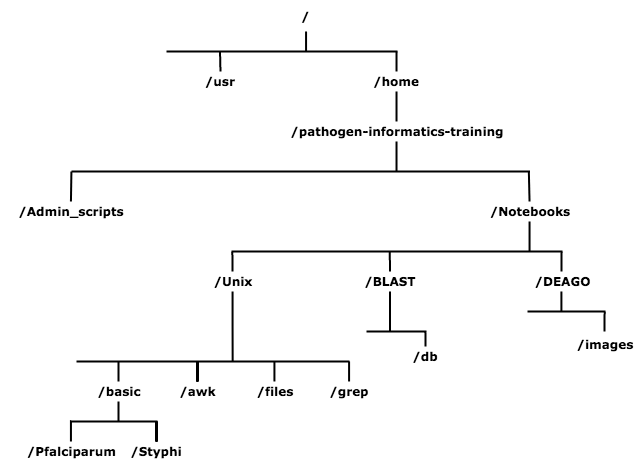
\includegraphics{basic/directory_structure.png}
\caption{Directory structure}
\end{figure}

    \hypertarget{pwd---find-where-you-are}{%
\subsection{pwd - find where you are}\label{pwd---find-where-you-are}}

The command \texttt{pwd} stands for print working directory. A
\textit{command} (also known as a \textit{program}) is something which tells
the computer to do something. Commands are therefore often the first
thing that you type into the terminal.

As described above, directories are arranged in a hierarchical
structure. To determine where you are in the hierarchy you can use the
\texttt{pwd} command to display the name of the current working
directory. The current working directory may be thought of as the
directory you are in, i.e.~your current position in the file-system
tree.

To find out where you are, type the following:

    \begin{tcolorbox}[breakable, size=fbox, boxrule=1pt, pad at break*=1mm,colback=cellbackground, colframe=cellborder]
\prompt{In}{incolor}{ }{\boxspacing}
\begin{Verbatim}[commandchars=\\\{\}]
\PY{n+nb}{pwd}
\end{Verbatim}
\end{tcolorbox}

    Remember that Unix is case sensitive, \texttt{PWD} is not the same as
\texttt{pwd}.

\texttt{pwd} will list each of the folders you would need to navigate
through to get from the \texttt{root} (top level directory) of the file
system to your current directory. This is sometimes refered to as your
`absolute path' to distinguish that it gives a complete route rather
than a `relative path' which tells you how to get from the current
working directory to another directory. More on that shortly.

    \hypertarget{ls---list-the-contents-of-a-directory}{%
\subsection{ls - list the contents of a
directory}\label{ls---list-the-contents-of-a-directory}}

The command \texttt{ls} stands for list. The \texttt{ls} command can be
used to list the contents of a directory.

To list the contents of your current working directory type:

    \begin{tcolorbox}[breakable, size=fbox, boxrule=1pt, pad at break*=1mm,colback=cellbackground, colframe=cellborder]
\prompt{In}{incolor}{ }{\boxspacing}
\begin{Verbatim}[commandchars=\\\{\}]
ls
\end{Verbatim}
\end{tcolorbox}

    You should see that there are 3 items in this directory.

To list the contents of a directory with extra information about the
items type:

    \begin{tcolorbox}[breakable, size=fbox, boxrule=1pt, pad at break*=1mm,colback=cellbackground, colframe=cellborder]
\prompt{In}{incolor}{ }{\boxspacing}
\begin{Verbatim}[commandchars=\\\{\}]
ls \PYZhy{}l
\end{Verbatim}
\end{tcolorbox}

    Instead of printing out a simple list, this should have printed out
additional information about each file. Note that there is a space
between the command \texttt{ls} and the \texttt{-l}. There is no space
between the dash and the letter l.

\texttt{-l} is our first example of an \textit{option}. Many commands have
options which change their behaviour but are not always required.

What do each of the columns represent? (file permissions, file owner,
group owner, size, date)

    To list all contents of a directory including hidden files and
directories (hidden files and directories are not shown by default and
are used to help important data from being deleted) type:

    \begin{tcolorbox}[breakable, size=fbox, boxrule=1pt, pad at break*=1mm,colback=cellbackground, colframe=cellborder]
\prompt{In}{incolor}{ }{\boxspacing}
\begin{Verbatim}[commandchars=\\\{\}]
ls \PYZhy{}a \PYZhy{}l
\end{Verbatim}
\end{tcolorbox}

    This is an example of a command which can take multiple options at the
same time.

How many hidden files and directories are there?

    Try the same command but with the \texttt{-h} option:

    \begin{tcolorbox}[breakable, size=fbox, boxrule=1pt, pad at break*=1mm,colback=cellbackground, colframe=cellborder]
\prompt{In}{incolor}{ }{\boxspacing}
\begin{Verbatim}[commandchars=\\\{\}]
ls \PYZhy{}alh
\end{Verbatim}
\end{tcolorbox}

    You'll also notice that we've combined \texttt{-a\ -l\ -h} into what
appears to be a single \texttt{-alh} option. It's almost always ok to do
this for options which are made up of a single dash followed by a single
letter.

What does the \texttt{-h} option do?

    To list the contents of the directory called Pfalciparum with extra
information type:

    \begin{tcolorbox}[breakable, size=fbox, boxrule=1pt, pad at break*=1mm,colback=cellbackground, colframe=cellborder]
\prompt{In}{incolor}{ }{\boxspacing}
\begin{Verbatim}[commandchars=\\\{\}]
ls \PYZhy{}l Pfalciparum/
\end{Verbatim}
\end{tcolorbox}

    In this case we gave \texttt{ls} an \textit{argument} describing the
\textit{relative path} to the directory \texttt{Pfalciparum} from our
current working directory. Arguments are very similar to options but
they often refer to things which are not prefixed with dashes.

How many files are there in this directory?

    \hypertarget{tab-completion}{%
\subsection{Tab completion}\label{tab-completion}}

Typing out directory or file names is really boring and you're likely to
make typos which will at best make your command fail with a strange
error and at worst overwrite some of your carefully crafted analysis.
\textit{Tab completion} is a trick which normally reduces this risk
significantly.

Instead of typing out \texttt{ls\ Pfalciparum/}, try typing
\texttt{ls\ P} and then press the \texttt{tab} key (instead of
\texttt{Enter}). The rest of the folder name should just appear. If you
have two files of directories with simiar names
(e.g.~\texttt{directory\_structure.png} and
\texttt{directory\_structure2.png}) then you might need to give your
terminal a bit of a hand to work out which one you want. In this case
you would type \texttt{ls\ -l\ d}, when you press \texttt{tab} the
terminal would read \texttt{ls\ -l\ directory\_structure}, you could
then type \texttt{2} followed by another \texttt{tab} and it would work
out that you meant \texttt{directory\_structure2.png}

    \hypertarget{file-permissions}{%
\subsection{File permissions}\label{file-permissions}}

Every file and directory have a set of permissions which restrict what
can be done with a file or directory.

\begin{itemize}
\tightlist
\item
  Read (r): permission to read from a file/directory
\item
  Write (w): permission to modify a file/directory
\item
  Execute (x): Tells the operating system that the file contains code
  for the computer to run, as opposed to a file of text which you open
  in a text editor.
\end{itemize}

Now open a new terminal on your computer and type the command that was
output by the previous cell followed by the enter key. The command will
look similar to this:The first set of permissions (characters 2,3,4)
refer to what the owner of the file can do, the second set of
permissions (5,6,7) refers to what members of the Unix group can do and
the third set of permissions (8,9,10) refers to what everyone else can
do.

    \hypertarget{cd---change-current-working-directory}{%
\subsection{cd - change current working
directory}\label{cd---change-current-working-directory}}

The command \texttt{cd} stands for change directory.

The \texttt{cd} command will move you from the current working directory
to another directory, in other words allow you to move up or down in the
directory hierarchy.

To move into the \texttt{Styphi} directory type the following. Note,
you'll remember this more easily if you type this rather than copying
and pasting. Also remember that you can use tab completion to save
typing all of it.

    \begin{tcolorbox}[breakable, size=fbox, boxrule=1pt, pad at break*=1mm,colback=cellbackground, colframe=cellborder]
\prompt{In}{incolor}{ }{\boxspacing}
\begin{Verbatim}[commandchars=\\\{\}]
\PY{n+nb}{cd} Styphi/
\end{Verbatim}
\end{tcolorbox}

    Now use the \texttt{pwd} command to check your location in the directory
hierarchy and the \texttt{ls} command to list the contents of this
directory.

    \begin{tcolorbox}[breakable, size=fbox, boxrule=1pt, pad at break*=1mm,colback=cellbackground, colframe=cellborder]
\prompt{In}{incolor}{ }{\boxspacing}
\begin{Verbatim}[commandchars=\\\{\}]
\PY{n+nb}{pwd}
\end{Verbatim}
\end{tcolorbox}

    \begin{tcolorbox}[breakable, size=fbox, boxrule=1pt, pad at break*=1mm,colback=cellbackground, colframe=cellborder]
\prompt{In}{incolor}{ }{\boxspacing}
\begin{Verbatim}[commandchars=\\\{\}]
ls
\end{Verbatim}
\end{tcolorbox}

    You should see that there are 3 files called: \texttt{Styphi.fa},
\texttt{Stypi.gff}, \texttt{Styphi.noseq.gff}

    \hypertarget{tips}{%
\subsection{Tips}\label{tips}}

There are some short cuts for referring to directories:

\begin{itemize}
\tightlist
\item
  . Current directory (one full stop)
\item
  .. Directory above in the hierarchy (two full stops)
\item
  \textasciitilde{} Home directory (tilde)
\item
  / Root of the file system (like C:~in Windows)
\end{itemize}

Try the following commands, what do they do?

    \begin{tcolorbox}[breakable, size=fbox, boxrule=1pt, pad at break*=1mm,colback=cellbackground, colframe=cellborder]
\prompt{In}{incolor}{ }{\boxspacing}
\begin{Verbatim}[commandchars=\\\{\}]
ls .
\end{Verbatim}
\end{tcolorbox}

    \begin{tcolorbox}[breakable, size=fbox, boxrule=1pt, pad at break*=1mm,colback=cellbackground, colframe=cellborder]
\prompt{In}{incolor}{ }{\boxspacing}
\begin{Verbatim}[commandchars=\\\{\}]
ls ..
\end{Verbatim}
\end{tcolorbox}

    \begin{tcolorbox}[breakable, size=fbox, boxrule=1pt, pad at break*=1mm,colback=cellbackground, colframe=cellborder]
\prompt{In}{incolor}{ }{\boxspacing}
\begin{Verbatim}[commandchars=\\\{\}]
ls \PYZti{}
\end{Verbatim}
\end{tcolorbox}

    As you may remember, \texttt{ls} will only \textit{list} what is in the
directories. To move to the directory, you need to use \texttt{cd}. Try
moving between directories a few times. Can you get into the
\texttt{Pfalciparum/} and then back into \texttt{Styphi/}? It might be
useful to look at Figure 1 when attempting this task.

    When you are finished moving between directories and have moved to the
Styphi directory type the command below.

    \begin{tcolorbox}[breakable, size=fbox, boxrule=1pt, pad at break*=1mm,colback=cellbackground, colframe=cellborder]
\prompt{In}{incolor}{ }{\boxspacing}
\begin{Verbatim}[commandchars=\\\{\}]
\PY{n+nb}{pwd}
\end{Verbatim}
\end{tcolorbox}

    It should return the result below, if not then you are not in the Styphi
directory.

    \texttt{/home/manager/pathogen-informatics-training/Notebooks/Unix/basic/Styphi}

    \hypertarget{cp---copy-a-file}{%
\subsection{cp - copy a file}\label{cp---copy-a-file}}

The command \texttt{cp} stands for copy.

The \texttt{cp} command will copy a file from one location to another
and you will end up with two copies of the file.

    To copy the file \texttt{Styphi.gff} to a new file called
\texttt{StyphiCT18.gff} type:

    \begin{tcolorbox}[breakable, size=fbox, boxrule=1pt, pad at break*=1mm,colback=cellbackground, colframe=cellborder]
\prompt{In}{incolor}{ }{\boxspacing}
\begin{Verbatim}[commandchars=\\\{\}]
cp Styphi.gff StyphiCT18.gff
\end{Verbatim}
\end{tcolorbox}

    Use \texttt{ls} to check the contents of the current directory for the
copied file:

    \begin{tcolorbox}[breakable, size=fbox, boxrule=1pt, pad at break*=1mm,colback=cellbackground, colframe=cellborder]
\prompt{In}{incolor}{ }{\boxspacing}
\begin{Verbatim}[commandchars=\\\{\}]
ls
\end{Verbatim}
\end{tcolorbox}

    \hypertarget{mv---move-a-file}{%
\subsection{mv - move a file}\label{mv---move-a-file}}

The \texttt{mv} command stand for move.

The \texttt{mv} command will move a file from one location to another.
This moves the file rather than copies it, therefore you end up with
only one file rather than two. When using the command, the path or
pathname is used to tell Unix where to find the file. You refer to files
in other directories by using the list of hierarchical names separated
by slashes. For example, the file called \texttt{StyphiCT18.gff} in the
directory \texttt{Styphi} has the path \texttt{Styphi/StyphiCT18}. If no
path is specified, Unix assumes that the file is in the current working
directory.

To move the file \texttt{StyphiCT18.gff} from the \texttt{Styphi}
directory to the current directory type:

    \begin{tcolorbox}[breakable, size=fbox, boxrule=1pt, pad at break*=1mm,colback=cellbackground, colframe=cellborder]
\prompt{In}{incolor}{ }{\boxspacing}
\begin{Verbatim}[commandchars=\\\{\}]
\PY{n+nb}{cd} ..
\end{Verbatim}
\end{tcolorbox}

    \begin{tcolorbox}[breakable, size=fbox, boxrule=1pt, pad at break*=1mm,colback=cellbackground, colframe=cellborder]
\prompt{In}{incolor}{ }{\boxspacing}
\begin{Verbatim}[commandchars=\\\{\}]
mv Styphi/StyphiCT18.gff .
\end{Verbatim}
\end{tcolorbox}

    Use the \texttt{ls} command to check the contents of the \texttt{Styphi}
directory and the current directory to see that \texttt{StyphiCT18.gff}
has been moved.

    \begin{tcolorbox}[breakable, size=fbox, boxrule=1pt, pad at break*=1mm,colback=cellbackground, colframe=cellborder]
\prompt{In}{incolor}{ }{\boxspacing}
\begin{Verbatim}[commandchars=\\\{\}]
ls Styphi
\end{Verbatim}
\end{tcolorbox}

    \begin{tcolorbox}[breakable, size=fbox, boxrule=1pt, pad at break*=1mm,colback=cellbackground, colframe=cellborder]
\prompt{In}{incolor}{ }{\boxspacing}
\begin{Verbatim}[commandchars=\\\{\}]
ls
\end{Verbatim}
\end{tcolorbox}

    \hypertarget{rm---delete-a-file}{%
\subsection{rm - delete a file}\label{rm---delete-a-file}}

The command \texttt{rm} stands for remove.

The \texttt{rm} command will delete a file permanently from your
computer so take care!

To remove the copy of the S. typhi file, called \texttt{StyphiCT18.gff}
type:

    \begin{tcolorbox}[breakable, size=fbox, boxrule=1pt, pad at break*=1mm,colback=cellbackground, colframe=cellborder]
\prompt{In}{incolor}{ }{\boxspacing}
\begin{Verbatim}[commandchars=\\\{\}]
rm StyphiCT18.gff
\end{Verbatim}
\end{tcolorbox}

    Use the \texttt{ls} command to check the contents of the current
directory to see that the file \texttt{StyphiCT18.gff} has been removed.

    \begin{tcolorbox}[breakable, size=fbox, boxrule=1pt, pad at break*=1mm,colback=cellbackground, colframe=cellborder]
\prompt{In}{incolor}{ }{\boxspacing}
\begin{Verbatim}[commandchars=\\\{\}]
ls
\end{Verbatim}
\end{tcolorbox}

    Unfortunately there is no ``recycle bin'' on the command line to recover
the file from, so you have to be careful!

    \hypertarget{find---find-a-file}{%
\subsection{find - find a file}\label{find---find-a-file}}

The \texttt{find} command can be used to find files matching a given
pattern. It can be used to recursively search the directory tree for a
specified name, seeking files and directories that match the given name.

    To find all files in the current directory and all its subdirectories
that end with the suffix gff:

    \begin{tcolorbox}[breakable, size=fbox, boxrule=1pt, pad at break*=1mm,colback=cellbackground, colframe=cellborder]
\prompt{In}{incolor}{ }{\boxspacing}
\begin{Verbatim}[commandchars=\\\{\}]
find . \PYZhy{}name *.gff
\end{Verbatim}
\end{tcolorbox}

    How many gff files did you find?

    To find all the subdirectories contained in the current directory type:

    \begin{tcolorbox}[breakable, size=fbox, boxrule=1pt, pad at break*=1mm,colback=cellbackground, colframe=cellborder]
\prompt{In}{incolor}{ }{\boxspacing}
\begin{Verbatim}[commandchars=\\\{\}]
find . \PYZhy{}type d
\end{Verbatim}
\end{tcolorbox}

    How many subdirectories did you find?

    \hypertarget{exercises}{%
\subsection{Exercises}\label{exercises}}

Many people panic when they are confronted with a Unix prompt! Don't!
All the commands you need to solve these exercises are provided above
and don't be afraid to make a mistake. If you get lost ask an
instructor. If you are a person skilled at Unix, be patient this is only
a short exercise.

To begin, open a terminal window and navigate to the \texttt{basic}
directory under the the \texttt{unix} directory (remember use the Unix
command \texttt{cd}) and then complete the exercise below.

\begin{enumerate}
\def\labelenumi{\arabic{enumi}.}
\tightlist
\item
  Use the \texttt{ls} command to show the contents of the \texttt{basic}
  directory.
\item
  How many files are there in the \texttt{Pfalciparum} directory?
\item
  What is the largest file in the \texttt{Pfalciparum} directory?
\item
  Move into the \texttt{Pfalciparum} directory.
\item
  How many files are there in the \texttt{fasta} directory?
\item
  Copy the file \texttt{Pfalciparum.bed} in the \texttt{Pfalciparum}
  directory into the \texttt{annotation} directory.
\item
  Move all the fasta files in the directory \texttt{Pfalciparum} to the
  \texttt{fasta} directory.
\item
  How many files are there in the \texttt{fasta} directory?
\item
  Use the \texttt{find} command to find all gff files in the
  \texttt{Unix} directory, how many files did you find?
\item
  Use the \texttt{find} command to find all the fasta files in the
  \texttt{Unix} directory, how many files did you find?
\end{enumerate}

    When you have completed these exercises move on to the next part of the
tutorial, \href{files.ipynb}{looking inside files}.


    % Add a bibliography block to the postdoc



\newpage





    \hypertarget{looking-inside-files}{%
\section{Looking inside files}\label{looking-inside-files}}

A common task is to look at the contents of a file. This can be achieved
using several different Unix commands, \texttt{less}, \texttt{head} and
\texttt{tail}. Let us consider some examples.

But first, change directory into the \texttt{files} directory. You may
find Figure 1 useful here as depending on the directory you are
currently in you may need to use a different command than the one shown
below.

    \begin{tcolorbox}[breakable, size=fbox, boxrule=1pt, pad at break*=1mm,colback=cellbackground, colframe=cellborder]
\prompt{In}{incolor}{ }{\boxspacing}
\begin{Verbatim}[commandchars=\\\{\}]
\PY{n+nb}{cd} ../files
\end{Verbatim}
\end{tcolorbox}

    \hypertarget{less}{%
\subsection{less}\label{less}}

The \texttt{less} command displays the contents of a specified file one
screen at a time. To test this command type the following command
followed by the enter key:

    \begin{tcolorbox}[breakable, size=fbox, boxrule=1pt, pad at break*=1mm,colback=cellbackground, colframe=cellborder]
\prompt{In}{incolor}{ }{\boxspacing}
\begin{Verbatim}[commandchars=\\\{\}]
less Styphi.gff
\end{Verbatim}
\end{tcolorbox}

    \begin{tcolorbox}[breakable, size=fbox, boxrule=1pt, pad at break*=1mm,colback=cellbackground, colframe=cellborder]
\prompt{In}{incolor}{ }{\boxspacing}
\begin{Verbatim}[commandchars=\\\{\}]
head Styphi.gff
\end{Verbatim}
\end{tcolorbox}

    The contents of the file \texttt{Styphi.gff} is displayed one screen at
a time, to view the next screen press the space bar. As
\texttt{Styphi.gff} is a large file this will take a while, therefore
you may want to escape or exit from this command. To do this, press the
q key, this kills the \texttt{less} command and returns you to the Unix
prompt. The \texttt{less} command can also scroll backwards if you hit
the \texttt{b} key. Another useful feature is the slash key, \texttt{/},
to search for an expression in the file. Try it, search for the gene
with locus tag t0038. What is the start and end position of this gene?

    \hypertarget{head-and-tail}{%
\subsection{head and tail}\label{head-and-tail}}

Sometimes you may just want to view the text at the beginning or the end
of a file, without having to display all of the file. The \texttt{head}
and \texttt{tail} commands can be used to do this.

    The \texttt{head} command displays the first ten lines of a file.

To look at the beginning of the fie \texttt{Styphi.gff} file type:

    \begin{tcolorbox}[breakable, size=fbox, boxrule=1pt, pad at break*=1mm,colback=cellbackground, colframe=cellborder]
\prompt{In}{incolor}{ }{\boxspacing}
\begin{Verbatim}[commandchars=\\\{\}]
head Styphi.gff
\end{Verbatim}
\end{tcolorbox}

    The \texttt{tail} command displays the last ten lines of a file.

To look at the end of \texttt{Styphi.gff} type:

    \begin{tcolorbox}[breakable, size=fbox, boxrule=1pt, pad at break*=1mm,colback=cellbackground, colframe=cellborder]
\prompt{In}{incolor}{ }{\boxspacing}
\begin{Verbatim}[commandchars=\\\{\}]
tail Styphi.gff
\end{Verbatim}
\end{tcolorbox}

    The amount of the file that is displayed can be increased by adding
extra options. To increase the number of lines viewed from 10 to 25 add
\texttt{-n\ 25} to the command:

    \begin{tcolorbox}[breakable, size=fbox, boxrule=1pt, pad at break*=1mm,colback=cellbackground, colframe=cellborder]
\prompt{In}{incolor}{ }{\boxspacing}
\begin{Verbatim}[commandchars=\\\{\}]
tail \PYZhy{}n \PY{l+m}{25} Styphi.gff
\end{Verbatim}
\end{tcolorbox}

    In this case you've given tail an option in two parts. In this case the
\texttt{-n} says that you want to specify the number of lines to show
and the \texttt{25} bit tells it how many. Unlike earlier when we merged
options like \texttt{ls\ -lha} together, it's not a good idea to merge
multiple two part options together because otherwise it is ambiguous
which value goes with which option.

The \texttt{-n} option is such a common option for \texttt{tail} and
\texttt{head} that it even has a shorthand: \texttt{-n\ 25} and
\texttt{-25} mean the same thing.

    \hypertarget{saving-time}{%
\subsection{Saving time}\label{saving-time}}

Saving time while typing may not seem important, but the longer that you
spend in front of a computer, the happier you will be if you can reduce
the time you spend at the keyboard.

\begin{itemize}
\item
  Pressing the up/down arrows will let you scroll through previous
  commands entered.
\item
  If you highlight some text, middle clicking on the mouse will paste it
  on the command line.
\item
  Tab completion doesn't just work on directory and file names, it also
  works on commands. Try it by typing \texttt{tai} and pressing yhe
  \texttt{tab} key.
\end{itemize}

Although tab completion works on commands and filenames, unfortunately
it does not work on options or other arguments.

    \hypertarget{getting-help-man}{%
\subsection{Getting help man}\label{getting-help-man}}

To obtain further information on any of the Unix commands introduced in
this course you can use the \texttt{man} command. For example, to get a
full description and examples of how to use the \texttt{tail} command
type the following command in a terminal window.

    \begin{tcolorbox}[breakable, size=fbox, boxrule=1pt, pad at break*=1mm,colback=cellbackground, colframe=cellborder]
\prompt{In}{incolor}{ }{\boxspacing}
\begin{Verbatim}[commandchars=\\\{\}]
man tail
\end{Verbatim}
\end{tcolorbox}

    There are several other useful commands that can be used to manipulate
and summarise information inside files and we will introduce some of
these next, \texttt{cat}, \texttt{sort}, \texttt{wc} and \texttt{uniq}.

    \hypertarget{writing-to-files}{%
\subsection{Writing to files}\label{writing-to-files}}

So far we've been running commands and outputting the results into the
terminal. That's obviously useful but what if you want to save the
results to another file?

Type this:

    \begin{tcolorbox}[breakable, size=fbox, boxrule=1pt, pad at break*=1mm,colback=cellbackground, colframe=cellborder]
\prompt{In}{incolor}{ }{\boxspacing}
\begin{Verbatim}[commandchars=\\\{\}]
head \PYZhy{}1 Styphi.gff \PYZgt{} first\PYZus{}Styphi\PYZus{}line.txt
\end{Verbatim}
\end{tcolorbox}

    It may look like nothing has happened. This is because the
\texttt{\textgreater{}} character has \textit{redirected} the output of
the \texttt{head} command. Instead of writing to the \textit{standard
output} (in this case your terminal) it sent the output into the file
\texttt{first\_Styphi\_line.txt}. Note that tab completion works for
\texttt{Styphi.gff} because it exists but doesn't work for
\texttt{first\_Styphi\_line.txt} because it doesn't exist yet.

    \hypertarget{cat}{%
\subsection{cat}\label{cat}}

\texttt{cat} is another way of reading files, but unlike \texttt{less}
it just throws the entire contents of the file to your standard output.
Try it on \texttt{first\_Styphi\_line.txt}

    \begin{tcolorbox}[breakable, size=fbox, boxrule=1pt, pad at break*=1mm,colback=cellbackground, colframe=cellborder]
\prompt{In}{incolor}{ }{\boxspacing}
\begin{Verbatim}[commandchars=\\\{\}]
cat first\PYZus{}Styphi\PYZus{}line.txt
\end{Verbatim}
\end{tcolorbox}

    We don't need \texttt{first\_Styphi\_line.txt} any more so delete it by
typing

    \begin{tcolorbox}[breakable, size=fbox, boxrule=1pt, pad at break*=1mm,colback=cellbackground, colframe=cellborder]
\prompt{In}{incolor}{ }{\boxspacing}
\begin{Verbatim}[commandchars=\\\{\}]
rm first\PYZus{}Styphi\PYZus{}line.txt
\end{Verbatim}
\end{tcolorbox}

    The \texttt{cat} command can also be given the names of multiple files,
one after the other and it will just output the contents of all files.
The order in which the files are displayed is determined by the order in
which they appear in the command line. You can use this concept and the
\texttt{\textgreater{}} symbol to join files together into a single
file.

Having looked at the beginning and end of the \texttt{Styphi.gff} file
you should notice that in the GFF file the annotation comes first, then
the DNA sequence at the end. If you had two separate files containing
the annotation and the DNA sequence, it is possible to concatenate or
join the two together to make a single file like the \texttt{Styphi.gff}
file you have just looked at.

For example, we have two separate files, \texttt{Styphi.noseq.gff} and
\texttt{Styphi.fa}, that contain the annotation and DNA sequence,
respectively for the Salmonella typhi CT18 genome. To join together
these files type:

    \begin{tcolorbox}[breakable, size=fbox, boxrule=1pt, pad at break*=1mm,colback=cellbackground, colframe=cellborder]
\prompt{In}{incolor}{ }{\boxspacing}
\begin{Verbatim}[commandchars=\\\{\}]
cat Styphi.noseq.gff Styphi.fa \PYZgt{} Styphi.concatenated.gff
\end{Verbatim}
\end{tcolorbox}

    The files \texttt{Styphi.noseq.gff} and \texttt{Styphi.fa} will be
joined together and written to a new file called
\texttt{Styphi.concatenated.gff}.

The \texttt{\textgreater{}} symbol in the command line directs the
output of the cat program to the designated file
\texttt{Styphi.concatenated.gff}. Use the command \texttt{ls} to check
for the presence of this file.

    \begin{tcolorbox}[breakable, size=fbox, boxrule=1pt, pad at break*=1mm,colback=cellbackground, colframe=cellborder]
\prompt{In}{incolor}{ }{\boxspacing}
\begin{Verbatim}[commandchars=\\\{\}]
ls
\end{Verbatim}
\end{tcolorbox}

    \hypertarget{wc---counting}{%
\subsection{wc - counting}\label{wc---counting}}

The command \texttt{wc} counts lines, words or characters.

There are two ways you could use it:

    \begin{tcolorbox}[breakable, size=fbox, boxrule=1pt, pad at break*=1mm,colback=cellbackground, colframe=cellborder]
\prompt{In}{incolor}{ }{\boxspacing}
\begin{Verbatim}[commandchars=\\\{\}]
wc \PYZhy{}l Styphi.gff
\end{Verbatim}
\end{tcolorbox}

    or

    \begin{tcolorbox}[breakable, size=fbox, boxrule=1pt, pad at break*=1mm,colback=cellbackground, colframe=cellborder]
\prompt{In}{incolor}{ }{\boxspacing}
\begin{Verbatim}[commandchars=\\\{\}]
cat Styphi.gff \PY{p}{|} wc \PYZhy{}l
\end{Verbatim}
\end{tcolorbox}

    Both give a similar answer. In the first example you tell \texttt{wc}
the file that you want it to review (\texttt{Styphi.gff}) and pass the
\texttt{-l} option to say that you're only interested in the number of
lines.

In the second example you use the \texttt{\textbar{}} symbol which is
also known as the \textit{pipe} symbol. This \textit{pipes} (sends) the
output of \texttt{cat\ Styphi.gff} into the input of \texttt{wc\ -l}.
This means that you can also use the same \texttt{wc} tool to count
other things. For example to count the number of files that are listed
by \texttt{ls} type:

    \begin{tcolorbox}[breakable, size=fbox, boxrule=1pt, pad at break*=1mm,colback=cellbackground, colframe=cellborder]
\prompt{In}{incolor}{ }{\boxspacing}
\begin{Verbatim}[commandchars=\\\{\}]
ls \PY{p}{|} wc \PYZhy{}l
\end{Verbatim}
\end{tcolorbox}

    You can connect as many commands as you want. For example, type:

    \begin{tcolorbox}[breakable, size=fbox, boxrule=1pt, pad at break*=1mm,colback=cellbackground, colframe=cellborder]
\prompt{In}{incolor}{ }{\boxspacing}
\begin{Verbatim}[commandchars=\\\{\}]
ls \PY{p}{|} grep \PY{l+s+s2}{\PYZdq{}.gff\PYZdq{}} \PY{p}{|} wc \PYZhy{}l
\end{Verbatim}
\end{tcolorbox}

    What does this command do? You will learn more about the \texttt{grep}
command later in this course.

    \hypertarget{sort---sorting-values}{%
\subsection{sort - sorting values}\label{sort---sorting-values}}

The \texttt{sort} lets you sort the contents of the input. When you sort
the input, lines with identical content end up next to each other in the
output. This is useful as the output can then be fed to the
\texttt{uniq} command (see below) to count the number of unique lines in
the input.

To sort the contents of a BED file type:

    \begin{tcolorbox}[breakable, size=fbox, boxrule=1pt, pad at break*=1mm,colback=cellbackground, colframe=cellborder]
\prompt{In}{incolor}{ }{\boxspacing}
\begin{Verbatim}[commandchars=\\\{\}]
sort Pfalciparum.bed
\end{Verbatim}
\end{tcolorbox}

    Now type:

    \begin{tcolorbox}[breakable, size=fbox, boxrule=1pt, pad at break*=1mm,colback=cellbackground, colframe=cellborder]
\prompt{In}{incolor}{ }{\boxspacing}
\begin{Verbatim}[commandchars=\\\{\}]
sort Pfalciparum.bed \PY{p}{|} head
\end{Verbatim}
\end{tcolorbox}

    \begin{tcolorbox}[breakable, size=fbox, boxrule=1pt, pad at break*=1mm,colback=cellbackground, colframe=cellborder]
\prompt{In}{incolor}{ }{\boxspacing}
\begin{Verbatim}[commandchars=\\\{\}]
sort Pfalciparum.bed \PY{p}{|} tail
\end{Verbatim}
\end{tcolorbox}

    To sort the contents of a BED file on position, type the following
command.

    \begin{tcolorbox}[breakable, size=fbox, boxrule=1pt, pad at break*=1mm,colback=cellbackground, colframe=cellborder]
\prompt{In}{incolor}{ }{\boxspacing}
\begin{Verbatim}[commandchars=\\\{\}]
sort \PYZhy{}k \PY{l+m}{2} \PYZhy{}n Pfalciparum.bed
\end{Verbatim}
\end{tcolorbox}

    The \texttt{sort} command can sort by multiple columns e.g.~1st column
and then 2nd column by specifying successive \texttt{-k} options in the
command. Type the following commands:

    \begin{tcolorbox}[breakable, size=fbox, boxrule=1pt, pad at break*=1mm,colback=cellbackground, colframe=cellborder]
\prompt{In}{incolor}{ }{\boxspacing}
\begin{Verbatim}[commandchars=\\\{\}]
sort \PYZhy{}k \PY{l+m}{2} \PYZhy{}n Pfalciparum.bed \PY{p}{|} head
\end{Verbatim}
\end{tcolorbox}

    \begin{tcolorbox}[breakable, size=fbox, boxrule=1pt, pad at break*=1mm,colback=cellbackground, colframe=cellborder]
\prompt{In}{incolor}{ }{\boxspacing}
\begin{Verbatim}[commandchars=\\\{\}]
sort \PYZhy{}k \PY{l+m}{2} \PYZhy{}n Pfalciparum.bed \PY{p}{|} tail
\end{Verbatim}
\end{tcolorbox}

    Why not have a look at the manual for \texttt{sort} to see what these
\texttt{-k} and \texttt{-n} options do? Remember that you can type
\texttt{/} followed by a search phrase, \texttt{n} to find the next
search hit, \texttt{N} to find the previous search hit and \texttt{q} to
exit.

    \begin{tcolorbox}[breakable, size=fbox, boxrule=1pt, pad at break*=1mm,colback=cellbackground, colframe=cellborder]
\prompt{In}{incolor}{ }{\boxspacing}
\begin{Verbatim}[commandchars=\\\{\}]
man sort
\end{Verbatim}
\end{tcolorbox}

    \hypertarget{uniq---finding-unique-values}{%
\subsection{uniq - finding unique
values}\label{uniq---finding-unique-values}}

The \texttt{uniq} command extracts unique lines from the input. It is
usually used in combination with \texttt{sort} to count unique values in
the input.

    To get the list of chromosomes in the Pfalciparum bed file type:

    \begin{tcolorbox}[breakable, size=fbox, boxrule=1pt, pad at break*=1mm,colback=cellbackground, colframe=cellborder]
\prompt{In}{incolor}{ }{\boxspacing}
\begin{Verbatim}[commandchars=\\\{\}]
awk \PY{l+s+s1}{\PYZsq{}\PYZob{} print \PYZdl{}1 \PYZcb{}\PYZsq{}} Pfalciparum.bed \PY{p}{|} sort \PY{p}{|} uniq
\end{Verbatim}
\end{tcolorbox}

    How many chromosomes are there? You will learn more about the
\texttt{awk} command later in this course.

Warning: \texttt{uniq} is really stupid; it can only spot that two lines
are the same if they are right next to one another. You therefore almost
always want to \texttt{sort} your input data before using \texttt{uniq}.

Do you understand how this command is working? Why not try building it
up piece by piece to see what it does?

    \begin{tcolorbox}[breakable, size=fbox, boxrule=1pt, pad at break*=1mm,colback=cellbackground, colframe=cellborder]
\prompt{In}{incolor}{ }{\boxspacing}
\begin{Verbatim}[commandchars=\\\{\}]
awk \PY{l+s+s1}{\PYZsq{}\PYZob{} print \PYZdl{}1 \PYZcb{}\PYZsq{}} Pfalciparum.bed \PY{p}{|} less
\end{Verbatim}
\end{tcolorbox}

    \begin{tcolorbox}[breakable, size=fbox, boxrule=1pt, pad at break*=1mm,colback=cellbackground, colframe=cellborder]
\prompt{In}{incolor}{ }{\boxspacing}
\begin{Verbatim}[commandchars=\\\{\}]
awk \PY{l+s+s1}{\PYZsq{}\PYZob{} print \PYZdl{}1 \PYZcb{}\PYZsq{}} Pfalciparum.bed \PY{p}{|} sort \PY{p}{|} less
\end{Verbatim}
\end{tcolorbox}

    \begin{tcolorbox}[breakable, size=fbox, boxrule=1pt, pad at break*=1mm,colback=cellbackground, colframe=cellborder]
\prompt{In}{incolor}{ }{\boxspacing}
\begin{Verbatim}[commandchars=\\\{\}]
awk \PY{l+s+s1}{\PYZsq{}\PYZob{} print \PYZdl{}1 \PYZcb{}\PYZsq{}} Pfalciparum.bed \PY{p}{|} sort \PY{p}{|} uniq \PY{p}{|} less
\end{Verbatim}
\end{tcolorbox}

    \hypertarget{exercises}{%
\subsection{Exercises}\label{exercises}}

Open up a new terminal window, navigate to the \texttt{files} directory
under the \texttt{unix} directory and complete the following exercises:

\begin{enumerate}
\def\labelenumi{\arabic{enumi}.}
\tightlist
\item
  Use the \texttt{head} command to extract the first 500 lines of the
  file \texttt{Styphi.gff} and store the output in a new file called
  \texttt{Styphi.500.gff}.
\item
  Use the \texttt{wc} command to count the number of lines in the
  \texttt{Pfalciparum.bed} file.
\item
  Use the \texttt{sort} command to sort the file
  \texttt{Pfalciparum.bed} on chromosome and then gene position.
\item
  Use the \texttt{uniq} command to count the number of features per
  chromosome in the \texttt{Pfalciparum.bed} file. Hint: use the man
  command to look at the options for the uniq command. Or peruse the
  \texttt{wc} or \texttt{grep} manuals.
\end{enumerate}

    When you have completed these exercises move on to the next part of the
tutorial, \href{grep.ipynb}{searching inside files with grep}.


    % Add a bibliography block to the postdoc



\newpage





    \hypertarget{searching-inside-files-with-grep}{%
\section{\texorpdfstring{Searching inside files with
\texttt{grep}}{Searching inside files with grep}}\label{searching-inside-files-with-grep}}

A common task is to extract information from large files. This can be
achieved using the Unix command \texttt{grep}, which stands for
``Globally search for a Regular Expression and Print''. The meaning of
this acronym will become clear later, when we discuss Regular
Expressions. First, we will consider simpler examples.

Before we start, change into the \texttt{grep} directory:

    \begin{tcolorbox}[breakable, size=fbox, boxrule=1pt, pad at break*=1mm,colback=cellbackground, colframe=cellborder]
\prompt{In}{incolor}{ }{\boxspacing}
\begin{Verbatim}[commandchars=\\\{\}]
\PY{n+nb}{cd} ../grep
\end{Verbatim}
\end{tcolorbox}

    \hypertarget{simple-pattern-matching}{%
\subsection{Simple pattern matching}\label{simple-pattern-matching}}

We will use a small example file (in ``BED'' format), which contains the
expression levels of some genes. This is a column-based file, with a tab
character between each column. There can be more than 10 columns, but
only the first three are required to be a valid file. The file format is
described in full here:
\url{http://genome.ucsc.edu/FAQ/FAQformat\#format1}. We will use the
first 5 columns:

\begin{enumerate}
\def\labelenumi{\arabic{enumi}.}
\tightlist
\item
  Sequence name
\item
  start position (starting from 0, not 1)
\item
  end position (starting from 0, not 1)
\item
  feature name
\item
  score (which is used to store the gene expression level in our
  examples).
\end{enumerate}

Here is the contents of the first example BED file used in this course:

    \begin{tcolorbox}[breakable, size=fbox, boxrule=1pt, pad at break*=1mm,colback=cellbackground, colframe=cellborder]
\prompt{In}{incolor}{ }{\boxspacing}
\begin{Verbatim}[commandchars=\\\{\}]
cat gene\PYZus{}expression.bed
\end{Verbatim}
\end{tcolorbox}

    In reality, such a file could contain 100,000s of lines, so that it is
not practical to read manually. Suppose we are interested in all the
genes from chromosome 2. We can find all these lines using grep:

    \begin{tcolorbox}[breakable, size=fbox, boxrule=1pt, pad at break*=1mm,colback=cellbackground, colframe=cellborder]
\prompt{In}{incolor}{ }{\boxspacing}
\begin{Verbatim}[commandchars=\\\{\}]
grep chr2 gene\PYZus{}expression.bed
\end{Verbatim}
\end{tcolorbox}

    This has shown us all the lines that contain the text or string
``chr2''.

We can use a pipe to then just extract the genes that are on the
positive strand, using grep a second time:

    \begin{tcolorbox}[breakable, size=fbox, boxrule=1pt, pad at break*=1mm,colback=cellbackground, colframe=cellborder]
\prompt{In}{incolor}{ }{\boxspacing}
\begin{Verbatim}[commandchars=\\\{\}]
grep chr2 gene\PYZus{}expression.bed \PY{p}{|} grep +
\end{Verbatim}
\end{tcolorbox}

    However, since \texttt{grep} is reporting a match to a string
\textit{anywhere} on a line, such simple searches can have undesired
consequences. For example, consider the result of doing a similar search
for all the genes in chromosome 1:

    \begin{tcolorbox}[breakable, size=fbox, boxrule=1pt, pad at break*=1mm,colback=cellbackground, colframe=cellborder]
\prompt{In}{incolor}{ }{\boxspacing}
\begin{Verbatim}[commandchars=\\\{\}]
grep chr1 gene\PYZus{}expression.bed
\end{Verbatim}
\end{tcolorbox}

    Oops! We found genes in chromosome 10, because ``chr1'' is a substring
(subset) of ``chr10''.

Or consider the following file, where the genes have unpredictable names
(which is not unusual for bioinformatics data).

    \begin{tcolorbox}[breakable, size=fbox, boxrule=1pt, pad at break*=1mm,colback=cellbackground, colframe=cellborder]
\prompt{In}{incolor}{ }{\boxspacing}
\begin{Verbatim}[commandchars=\\\{\}]
cat gene\PYZus{}expression\PYZus{}sneaky.bed
\end{Verbatim}
\end{tcolorbox}

    Now we try to find genes on chromosome 1 that are on the negative
strand. We put the minus sign in quotes, to stop Unix interpreting this
as an option to \texttt{grep}, as opposed to the string we are searching
for:

    \begin{tcolorbox}[breakable, size=fbox, boxrule=1pt, pad at break*=1mm,colback=cellbackground, colframe=cellborder]
\prompt{In}{incolor}{ }{\boxspacing}
\begin{Verbatim}[commandchars=\\\{\}]
grep chr1 gene\PYZus{}expression\PYZus{}sneaky.bed \PY{p}{|} grep \PY{l+s+s1}{\PYZsq{}\PYZhy{}\PYZsq{}}
\end{Verbatim}
\end{tcolorbox}

    The extra lines are found by \texttt{grep} because of matches in columns
we were not expecting to match. Remember, \texttt{grep} is reporting
these lines because they each contain the strings ``chr1'' and ``-''
\textit{somewhere}.

We need a way to make searching with \texttt{grep} more specific.

\hypertarget{regular-expressions}{%
\subsection{Regular expressions}\label{regular-expressions}}

Regular expressions provide the solution to the above problems. They are
a way of defining more specific patterns to search for.

\hypertarget{matching-the-start-and-end-of-lines}{%
\subsubsection{Matching the start and end of
lines}\label{matching-the-start-and-end-of-lines}}

First, we can specify that a match must be at the start of a line using
the symbol ``\texttt{\^{}}'', which means ``start of line''. Without the
\texttt{\^{}}, we find any match to ``chr1'':

    \begin{tcolorbox}[breakable, size=fbox, boxrule=1pt, pad at break*=1mm,colback=cellbackground, colframe=cellborder]
\prompt{In}{incolor}{ }{\boxspacing}
\begin{Verbatim}[commandchars=\\\{\}]
grep chr1 gene\PYZus{}expression\PYZus{}sneaky.bed
\end{Verbatim}
\end{tcolorbox}

    However, notice the effect of searching for \texttt{\^{}chr1} instead.
Note that we put the regular expression in quotes, to avoid Unix errors.
Not using quotes may or may not give an error, but it is safest to use
quotes for anything but the simplest of searches.

    \begin{tcolorbox}[breakable, size=fbox, boxrule=1pt, pad at break*=1mm,colback=cellbackground, colframe=cellborder]
\prompt{In}{incolor}{ }{\boxspacing}
\begin{Verbatim}[commandchars=\\\{\}]
grep \PY{l+s+s1}{\PYZsq{}\PYZca{}chr1\PYZsq{}} gene\PYZus{}expression\PYZus{}sneaky.bed
\end{Verbatim}
\end{tcolorbox}

    Good! We have removed the match to the badly-named gene ``chr11.gene1'',
which is on chromosome 8. Now we want to avoid matching chromosomes 10
and 11. This can be done by also looking for a ``tab'' character, which
is represented by writing \texttt{\textbackslash{}t}. For technical
reasons, which are beyond the scope of this course, we must also put a
dollar sign before the quotes to make any search involving a tab
character work.

    \begin{tcolorbox}[breakable, size=fbox, boxrule=1pt, pad at break*=1mm,colback=cellbackground, colframe=cellborder]
\prompt{In}{incolor}{ }{\boxspacing}
\begin{Verbatim}[commandchars=\\\{\}]
grep \PY{l+s+s1}{\PYZdl{}\PYZsq{}\PYZca{}chr1\PYZbs{}t\PYZsq{}} gene\PYZus{}expression\PYZus{}sneaky.bed
\end{Verbatim}
\end{tcolorbox}

    To find the genes on the negative strand, all that remains is to match a
minus sign at the \textit{end} of the line (so that we do not find
``sneaky-gene3''). We can do this using the dollar ``\texttt{\$}'',
which means ``end of line''.

    \begin{tcolorbox}[breakable, size=fbox, boxrule=1pt, pad at break*=1mm,colback=cellbackground, colframe=cellborder]
\prompt{In}{incolor}{ }{\boxspacing}
\begin{Verbatim}[commandchars=\\\{\}]
grep \PY{l+s+s1}{\PYZdl{}\PYZsq{}\PYZca{}chr1\PYZbs{}t\PYZsq{}} gene\PYZus{}expression\PYZus{}sneaky.bed \PY{p}{|} grep \PY{l+s+s1}{\PYZsq{}\PYZbs{}\PYZhy{}\PYZdl{}\PYZsq{}}
\end{Verbatim}
\end{tcolorbox}

    \hypertarget{wildcards-and-alphabets}{%
\subsubsection{Wildcards and alphabets}\label{wildcards-and-alphabets}}

Another special character in regular expressions is the dot: ``.''. This
stands for any single character. For example, this finds all matches to
chromosomes 1-9, and chromosomes X and Y:

    \begin{tcolorbox}[breakable, size=fbox, boxrule=1pt, pad at break*=1mm,colback=cellbackground, colframe=cellborder]
\prompt{In}{incolor}{ }{\boxspacing}
\begin{Verbatim}[commandchars=\\\{\}]
grep \PY{l+s+s1}{\PYZdl{}\PYZsq{}\PYZca{}chr.\PYZbs{}t\PYZsq{}} gene\PYZus{}expression.bed
\end{Verbatim}
\end{tcolorbox}

    In fact, the earlier command that found all genes on chromosome 1 that
are on the negative strand, could be found with a single call to
\texttt{grep} instead of two calls piped together. To do this, we need a
regular expression that finds lines that:

\begin{itemize}
\tightlist
\item
  start with chr1, then a tab character
\item
  end with a minus
\item
  have arbitrary characters between.
\end{itemize}

The asterisk ``*'' has a special meaning: it says to match any number
(including zero) of whatever character is before the *. For example, the
regular expression `AC*G' will match AG, ACG, ACCG, etc. The simpler,
improved command is:

    \begin{tcolorbox}[breakable, size=fbox, boxrule=1pt, pad at break*=1mm,colback=cellbackground, colframe=cellborder]
\prompt{In}{incolor}{ }{\boxspacing}
\begin{Verbatim}[commandchars=\\\{\}]
grep \PY{l+s+s1}{\PYZdl{}\PYZsq{}\PYZca{}chr1\PYZbs{}t.*\PYZhy{}\PYZdl{}\PYZsq{}} gene\PYZus{}expression\PYZus{}sneaky.bed
\end{Verbatim}
\end{tcolorbox}

    As well as matching any character using a dot, we can define any list of
characters to match, using square brackets. For example, {[}12X{]} means
match a 1, 2, or an X. This can be used to find all genes from
chromosomes 1, 2 and X:

    \begin{tcolorbox}[breakable, size=fbox, boxrule=1pt, pad at break*=1mm,colback=cellbackground, colframe=cellborder]
\prompt{In}{incolor}{ }{\boxspacing}
\begin{Verbatim}[commandchars=\\\{\}]
grep \PY{l+s+s1}{\PYZdl{}\PYZsq{}\PYZca{}chr[12X]\PYZbs{}t\PYZsq{}} gene\PYZus{}expression.bed
\end{Verbatim}
\end{tcolorbox}

    Or just the autosomes may be of interest. To do this we introduce two
new features:

\begin{itemize}
\tightlist
\item
  Ranges can be given in square brackets, for example {[}1-5{]} will
  match 1, 2, 3, 4 or 5.
\item
  The plus sign ``+'' has a special meaning that is similar to ``*''.
  Instead of any number of matches (including zero), it looks for at
  least one match. To avoid simply matching a plus sign, it must be
  preceded by a backslash: ``\textbackslash+''. For example, the regular
  expression `AC\textbackslash+G' will match ACG, ACCG, ACCCG etc (but
  will not match AG).
\end{itemize}

Warning: Adding a backslash is often called \textit{escaping}
(e.g.~\textit{escape the plus symbol}). Depending on the software you're
using (and the options you give it), you may need to escape the symbol
to indicate that you want its special regex meaning (e.g.~multiple
copies of the last character please) or its literal meaning (e.g.~give
me a `+' symbol please). If your command isn't working as you expect,
try playing with these options and always test your regular expression
before assuming it gave you the right answer.

The command to find the autosomes is:

    \begin{tcolorbox}[breakable, size=fbox, boxrule=1pt, pad at break*=1mm,colback=cellbackground, colframe=cellborder]
\prompt{In}{incolor}{ }{\boxspacing}
\begin{Verbatim}[commandchars=\\\{\}]
grep \PY{l+s+s1}{\PYZdl{}\PYZsq{}\PYZca{}chr[0\PYZhy{}9]\PYZbs{}+\PYZbs{}t\PYZsq{}} gene\PYZus{}expression.bed
\end{Verbatim}
\end{tcolorbox}

    \hypertarget{other-grep-options}{%
\subsection{\texorpdfstring{Other \texttt{grep}
options}{Other grep options}}\label{other-grep-options}}

The Unix command \texttt{grep} and regular expressions are extremely
powerful and we have only scratched the surface of what they can do.
Take a look at the manual (by typing \texttt{man\ grep}) to get an idea.
A few particularly useful options are discussed below.

    \begin{tcolorbox}[breakable, size=fbox, boxrule=1pt, pad at break*=1mm,colback=cellbackground, colframe=cellborder]
\prompt{In}{incolor}{ }{\boxspacing}
\begin{Verbatim}[commandchars=\\\{\}]
man grep
\end{Verbatim}
\end{tcolorbox}

    \hypertarget{counting-matches}{%
\subsubsection{Counting matches}\label{counting-matches}}

A common use-case is counting matches within files. Instead of output
each matching line, the option ``\texttt{-c}'' tells \texttt{grep} to
report the number of lines that matched. For example, the number of
genes in the autosomes in the above example can be found by simply
adding \texttt{-c} to the command.

    \begin{tcolorbox}[breakable, size=fbox, boxrule=1pt, pad at break*=1mm,colback=cellbackground, colframe=cellborder]
\prompt{In}{incolor}{ }{\boxspacing}
\begin{Verbatim}[commandchars=\\\{\}]
grep \PYZhy{}c \PY{l+s+s1}{\PYZdl{}\PYZsq{}\PYZca{}chr[0\PYZhy{}9]\PYZbs{}+\PYZbs{}t\PYZsq{}} gene\PYZus{}expression.bed
\end{Verbatim}
\end{tcolorbox}

    \hypertarget{case-sensitivity}{%
\subsubsection{Case sensitivity}\label{case-sensitivity}}

By default, \texttt{grep} is case-sensitive. It can be useful to ignore
the distinction between upper and lower case using the option
``\texttt{-i}''. Suppose we have a file of sequences, and want to find
the sequences that contain the string ACGT. It is not unusual to come
across files that have a mix of upper and lower case nucleotides.
Consider this FASTA file:

    \begin{tcolorbox}[breakable, size=fbox, boxrule=1pt, pad at break*=1mm,colback=cellbackground, colframe=cellborder]
\prompt{In}{incolor}{ }{\boxspacing}
\begin{Verbatim}[commandchars=\\\{\}]
cat sequences.fasta
\end{Verbatim}
\end{tcolorbox}

    A simple search for ACGT will not return all the results:

    \begin{tcolorbox}[breakable, size=fbox, boxrule=1pt, pad at break*=1mm,colback=cellbackground, colframe=cellborder]
\prompt{In}{incolor}{ }{\boxspacing}
\begin{Verbatim}[commandchars=\\\{\}]
grep ACGT sequences.fasta
\end{Verbatim}
\end{tcolorbox}

    However, making the search case-insensitive solves the problem.

    \begin{tcolorbox}[breakable, size=fbox, boxrule=1pt, pad at break*=1mm,colback=cellbackground, colframe=cellborder]
\prompt{In}{incolor}{ }{\boxspacing}
\begin{Verbatim}[commandchars=\\\{\}]
grep \PYZhy{}i ACGT sequences.fasta
\end{Verbatim}
\end{tcolorbox}

    \hypertarget{searching-in-more-than-one-file}{%
\subsubsection{Searching in more than one
file}\label{searching-in-more-than-one-file}}

So far, we have restricted to searches in one file, but \texttt{grep}
can be given a list of files in which to search. As an example, we are
given three files called \texttt{list\_example.1},
\texttt{list\_example.2}, and \texttt{list\_example.3}. They are simple
lists of genes, for illustrative purposes. For example, the first file
looks like this:

    \begin{tcolorbox}[breakable, size=fbox, boxrule=1pt, pad at break*=1mm,colback=cellbackground, colframe=cellborder]
\prompt{In}{incolor}{ }{\boxspacing}
\begin{Verbatim}[commandchars=\\\{\}]
cat list\PYZus{}example.1
\end{Verbatim}
\end{tcolorbox}

    Which files contain ``gene1''?

    \begin{tcolorbox}[breakable, size=fbox, boxrule=1pt, pad at break*=1mm,colback=cellbackground, colframe=cellborder]
\prompt{In}{incolor}{ }{\boxspacing}
\begin{Verbatim}[commandchars=\\\{\}]
grep \PY{l+s+s1}{\PYZsq{}\PYZca{}gene1\PYZdl{}\PYZsq{}} list\PYZus{}example.1 list\PYZus{}example.2
\end{Verbatim}
\end{tcolorbox}

    gene1 only appears in the file \texttt{list\_example.1}. The output
format of \texttt{grep} has now changed, because it was given a list of
files. The format is:

\begin{itemize}
\tightlist
\item
  filename:line\_that\_matches
\end{itemize}

ie, the name of the file has been added to the start of each matching
line.

For convenience, there's also a way of specifying all of the list
examples:

    \begin{tcolorbox}[breakable, size=fbox, boxrule=1pt, pad at break*=1mm,colback=cellbackground, colframe=cellborder]
\prompt{In}{incolor}{ }{\boxspacing}
\begin{Verbatim}[commandchars=\\\{\}]
\PY{n+nb}{echo} list\PYZus{}example.*
\end{Verbatim}
\end{tcolorbox}

    \begin{tcolorbox}[breakable, size=fbox, boxrule=1pt, pad at break*=1mm,colback=cellbackground, colframe=cellborder]
\prompt{In}{incolor}{ }{\boxspacing}
\begin{Verbatim}[commandchars=\\\{\}]
grep \PY{l+s+s1}{\PYZsq{}\PYZca{}gene1\PYZdl{}\PYZsq{}} list\PYZus{}example.*
\end{Verbatim}
\end{tcolorbox}

    How about gene42?

    \begin{tcolorbox}[breakable, size=fbox, boxrule=1pt, pad at break*=1mm,colback=cellbackground, colframe=cellborder]
\prompt{In}{incolor}{ }{\boxspacing}
\begin{Verbatim}[commandchars=\\\{\}]
grep \PY{l+s+s1}{\PYZsq{}\PYZca{}gene42\PYZdl{}\PYZsq{}} list\PYZus{}example.*
\end{Verbatim}
\end{tcolorbox}

    gene42 appears once in \texttt{list\_example.2} and twice in
\texttt{list\_example.3}.

    \hypertarget{inverting-matches}{%
\subsubsection{Inverting matches}\label{inverting-matches}}

By default, \texttt{grep} reports all lines that do match the regular
expression. Sometimes it is useful to filter a file, by reporting lines
that \textit{do not} match the regular expression. Using the option
``\texttt{-v}'' makes \texttt{grep} ``invert'' the output. For example,
we could exclude genes from autosomes in the BED file from earlier.

    \begin{tcolorbox}[breakable, size=fbox, boxrule=1pt, pad at break*=1mm,colback=cellbackground, colframe=cellborder]
\prompt{In}{incolor}{ }{\boxspacing}
\begin{Verbatim}[commandchars=\\\{\}]
grep \PYZhy{}v \PY{l+s+s1}{\PYZdl{}\PYZsq{}\PYZca{}chr[0\PYZhy{}9]\PYZbs{}+\PYZbs{}t\PYZsq{}} gene\PYZus{}expression.bed
\end{Verbatim}
\end{tcolorbox}

    \hypertarget{replacing-matches-to-regular-expressions}{%
\subsection{Replacing matches to regular
expressions}\label{replacing-matches-to-regular-expressions}}

Finally, we show how to replace every match to a regular expression with
something else, using the command ``\texttt{sed}''. The general form of
this is:

\begin{verbatim}
sed 's/regular expression/new string/' input_file
\end{verbatim}

This will output a new version of the input file, with each match to the
regular expression replaced with ``\texttt{new\ string}''. For example:

    \begin{tcolorbox}[breakable, size=fbox, boxrule=1pt, pad at break*=1mm,colback=cellbackground, colframe=cellborder]
\prompt{In}{incolor}{ }{\boxspacing}
\begin{Verbatim}[commandchars=\\\{\}]
sed \PY{l+s+s1}{\PYZsq{}s/\PYZca{}chr/chromosome/\PYZsq{}} gene\PYZus{}expression.bed
\end{Verbatim}
\end{tcolorbox}

    \hypertarget{exercises}{%
\subsection{Exercises}\label{exercises}}

The following exercises all use the FASTA file \texttt{exercises.fasta}.
Before starting the exercises, open a new terminal and navigate to the
\texttt{grep} directory, which contains \texttt{exercises.fasta}.

Use \texttt{grep} to find the answers. Hint: some questions require you
to use \texttt{grep} twice, and possibly some other Unix commands.

\begin{enumerate}
\def\labelenumi{\arabic{enumi}.}
\tightlist
\item
  Make a \texttt{grep} command that outputs just the lines with the
  sequence names.
\item
  How many sequences are in the file?
\item
  Do any sequence names have spaces in them? What are their names?
\item
  Make a \texttt{grep} command that outputs just the lines with the
  sequences, not the names.
\item
  How many sequences contain unknown bases (an ``n'' or ``N'')?
\item
  Are there any sequences that contain non-nucleotides (something other
  than A, C, G, T or N)?
\item
  How many sequences contain the 5' cut site GCWGC (where W can be an A
  or T) for the restriction enzyme AceI?
\item
  Are there any sequences that have the same name? You do not need to
  find the actual repeated names, just whether any names are repeated.
  (Hint: it may be easier to first discover how many unique names there
  are).
\end{enumerate}

    When you have completed the exercises move on to the next part of the
tutorial, \href{awk.ipynb}{file processing with AWK}.


    % Add a bibliography block to the postdoc



\newpage





    \hypertarget{file-processing-with-awk}{%
\section{File processing with AWK}\label{file-processing-with-awk}}

AWK is a programming language named after the initials of its three
inventors: Alfred \textbf{A}ho, Peter \textbf{W}einberger, and Brian
\textbf{K}ernighan. AWK is incredibly powerful at processing files,
particularly column-based files, which are commonplace in
Bioinformatics. For example, BED, GFF, and SAM files.

Although long programs, put into a separate file, can be written using
AWK, we will use it directly on the command line. Effectively, these are
very short AWK programs, often called ``one-liners''.

Before we start, change into the \texttt{awk} directory:

    \begin{tcolorbox}[breakable, size=fbox, boxrule=1pt, pad at break*=1mm,colback=cellbackground, colframe=cellborder]
\prompt{In}{incolor}{ }{\boxspacing}
\begin{Verbatim}[commandchars=\\\{\}]
\PY{n+nb}{cd} ../awk
\end{Verbatim}
\end{tcolorbox}

    \hypertarget{extracting-columns-from-files}{%
\subsection{Extracting columns from
files}\label{extracting-columns-from-files}}

\texttt{awk} reads a file line-by-line, splitting each line into
columns. This makes it easy to do simple things like extract a column
from a file. We will use the following GFF file for our examples.

    \begin{tcolorbox}[breakable, size=fbox, boxrule=1pt, pad at break*=1mm,colback=cellbackground, colframe=cellborder]
\prompt{In}{incolor}{ }{\boxspacing}
\begin{Verbatim}[commandchars=\\\{\}]
cat genes.gff
\end{Verbatim}
\end{tcolorbox}

    The columns in the GFF file are separated by tabs and have the following
meanings:

\begin{enumerate}
\def\labelenumi{\arabic{enumi}.}
\tightlist
\item
  Sequence name
\item
  Source - the name of the program that made the feature
\item
  Feature - the type of feature, for example gene or CDS
\item
  Start position
\item
  Stop position
\item
  Score
\item
  Strand (+ or -)
\item
  Frame (0, 1, or 2)
\item
  Optional extra information, in the form
  key1=value1;key2=value2;\ldots{}
\end{enumerate}

The score, strand, and frame can be set to `.' if it is not relevant for
that feature. The final column 9 may or may not be present and could
contain any number of key, value pairs.

We can use \texttt{awk} to just print the first column of the file.
\texttt{awk} calls the columns \texttt{\$1}, \texttt{\$2}, \ldots{} etc,
and the complete line is called \texttt{\$0}. Try

    \begin{tcolorbox}[breakable, size=fbox, boxrule=1pt, pad at break*=1mm,colback=cellbackground, colframe=cellborder]
\prompt{In}{incolor}{ }{\boxspacing}
\begin{Verbatim}[commandchars=\\\{\}]
awk \PYZhy{}F\PY{l+s+s2}{\PYZdq{}\PYZbs{}t\PYZdq{}} \PY{l+s+s1}{\PYZsq{}\PYZob{}print \PYZdl{}1\PYZcb{}\PYZsq{}} genes.gff
\end{Verbatim}
\end{tcolorbox}

    A little explanation is needed.

\begin{itemize}
\tightlist
\item
  The option \texttt{-F"\textbackslash{}t"} was needed to tell
  \texttt{awk} that the columns are separated by tabs (more on this
  later).
\item
  For each line of the file, \texttt{awk} does what is inside the curly
  brackets. In this case, we simply print the first column.
\end{itemize}

The repeated chromosome names are not nice. It is more likely to want to
know just the unique names, which can be found by piping into the Unix
command \texttt{sort}.

    \begin{tcolorbox}[breakable, size=fbox, boxrule=1pt, pad at break*=1mm,colback=cellbackground, colframe=cellborder]
\prompt{In}{incolor}{ }{\boxspacing}
\begin{Verbatim}[commandchars=\\\{\}]
awk \PYZhy{}F\PY{l+s+s2}{\PYZdq{}\PYZbs{}t\PYZdq{}} \PY{l+s+s1}{\PYZsq{}\PYZob{}print \PYZdl{}1\PYZcb{}\PYZsq{}} genes.gff \PY{p}{|} sort \PYZhy{}u
\end{Verbatim}
\end{tcolorbox}

    \hypertarget{filtering-the-input-file}{%
\subsection{Filtering the input file}\label{filtering-the-input-file}}

Similarly to \texttt{grep}, \texttt{awk} can be used to filter out lines
of a file. However, since \texttt{awk} is column-based, it makes it easy
to filter based on properties of any columns of interest. The filtering
criteria can be added before the braces. For example, the following
extracts just chromosome 1 from the file.

    \begin{tcolorbox}[breakable, size=fbox, boxrule=1pt, pad at break*=1mm,colback=cellbackground, colframe=cellborder]
\prompt{In}{incolor}{ }{\boxspacing}
\begin{Verbatim}[commandchars=\\\{\}]
awk \PYZhy{}F\PY{l+s+s2}{\PYZdq{}\PYZbs{}t\PYZdq{}} \PY{l+s+s1}{\PYZsq{}\PYZdl{}1==\PYZdq{}chr1\PYZdq{} \PYZob{}print \PYZdl{}0\PYZcb{}\PYZsq{}} genes.gff
\end{Verbatim}
\end{tcolorbox}

    There are two important things to note from the above command:

\begin{enumerate}
\def\labelenumi{\arabic{enumi}.}
\tightlist
\item
  \texttt{\$1=="chr1"} means that column 1 must be \textit{exactly} equal
  to ``chr1''. This means that ``chr10'' is not found.
\item
  The ``\texttt{\{print\ \$0\}}'' part only happens when the first
  column is equal to ``chr1'', otherwise \texttt{awk} does nothing (the
  line gets ignored).
\end{enumerate}

Awk commands are made up of two parts, a \textit{pattern}
(e.g.~\texttt{\$1=="chr1"}) and an \textit{action}
(e.g.~\texttt{print\ \$0}) which is contained in curly braces. The
\textit{pattern} defines which lines the \textit{action} is applied to.

In fact, the action (the part in curly braces) can be omitted in this
example. \texttt{awk} assumes that you want to print the whole line,
unless it is told otherwise. This gives a simple method of filtering
based on columns.

    \begin{tcolorbox}[breakable, size=fbox, boxrule=1pt, pad at break*=1mm,colback=cellbackground, colframe=cellborder]
\prompt{In}{incolor}{ }{\boxspacing}
\begin{Verbatim}[commandchars=\\\{\}]
awk \PYZhy{}F\PY{l+s+s2}{\PYZdq{}\PYZbs{}t\PYZdq{}} \PY{l+s+s1}{\PYZsq{}\PYZdl{}1==\PYZdq{}chr1\PYZdq{}\PYZsq{}} genes.gff
\end{Verbatim}
\end{tcolorbox}

    You might remember using another of awk's defaults in a previous
exercise. In that example we supplied an action but no pattern. In this
case, awk assumes that you want to apply the action to every line in the
file. For example:

    \begin{tcolorbox}[breakable, size=fbox, boxrule=1pt, pad at break*=1mm,colback=cellbackground, colframe=cellborder]
\prompt{In}{incolor}{ }{\boxspacing}
\begin{Verbatim}[commandchars=\\\{\}]
awk \PYZhy{}F\PY{l+s+s2}{\PYZdq{}\PYZbs{}t\PYZdq{}} \PY{l+s+s1}{\PYZsq{}\PYZob{}print \PYZdl{}1\PYZcb{}\PYZsq{}} genes.gff
\end{Verbatim}
\end{tcolorbox}

    Multiple patterns can be combined using ``\texttt{\&\&}'' to mean
``and''. For example, to find just the genes from chromosome 1:

    \begin{tcolorbox}[breakable, size=fbox, boxrule=1pt, pad at break*=1mm,colback=cellbackground, colframe=cellborder]
\prompt{In}{incolor}{ }{\boxspacing}
\begin{Verbatim}[commandchars=\\\{\}]
awk \PYZhy{}F\PY{l+s+s2}{\PYZdq{}\PYZbs{}t\PYZdq{}} \PY{l+s+s1}{\PYZsq{}\PYZdl{}1==\PYZdq{}chr1\PYZdq{} \PYZam{}\PYZam{} \PYZdl{}3==\PYZdq{}gene\PYZdq{}\PYZsq{}} genes.gff
\end{Verbatim}
\end{tcolorbox}

    The entire line need not be printed (remember, if not specified,
\texttt{awk} assumes a \texttt{print\ \$0}). Suppose we want only the
sources of the genes on chromosome 1:

    \begin{tcolorbox}[breakable, size=fbox, boxrule=1pt, pad at break*=1mm,colback=cellbackground, colframe=cellborder]
\prompt{In}{incolor}{ }{\boxspacing}
\begin{Verbatim}[commandchars=\\\{\}]
awk \PYZhy{}F\PY{l+s+s2}{\PYZdq{}\PYZbs{}t\PYZdq{}} \PY{l+s+s1}{\PYZsq{}\PYZdl{}1==\PYZdq{}chr1\PYZdq{} \PYZam{}\PYZam{} \PYZdl{}3==\PYZdq{}gene\PYZdq{} \PYZob{}print \PYZdl{}2\PYZcb{}\PYZsq{}} genes.gff \PY{p}{|} sort \PYZhy{}u
\end{Verbatim}
\end{tcolorbox}

    Similarly to using ``\texttt{\&\&}'' for ``and'', there is
``\texttt{\textbar{}\textbar{}}'' to mean ``or''. To find features that
are repeats or made by the tool ``source2'':

    \begin{tcolorbox}[breakable, size=fbox, boxrule=1pt, pad at break*=1mm,colback=cellbackground, colframe=cellborder]
\prompt{In}{incolor}{ }{\boxspacing}
\begin{Verbatim}[commandchars=\\\{\}]
awk \PYZhy{}F\PY{l+s+s2}{\PYZdq{}\PYZbs{}t\PYZdq{}} \PY{l+s+s1}{\PYZsq{}\PYZdl{}2==\PYZdq{}source2\PYZdq{} || \PYZdl{}3==\PYZdq{}repeat\PYZdq{}\PYZsq{}} genes.gff
\end{Verbatim}
\end{tcolorbox}

    So far, we have only used strings for the filtering. Numbers can also be
used. We could ask \texttt{awk} to return all the genes on chromosome 1
that start before position 1100:

    \begin{tcolorbox}[breakable, size=fbox, boxrule=1pt, pad at break*=1mm,colback=cellbackground, colframe=cellborder]
\prompt{In}{incolor}{ }{\boxspacing}
\begin{Verbatim}[commandchars=\\\{\}]
awk \PYZhy{}F\PY{l+s+s2}{\PYZdq{}\PYZbs{}t\PYZdq{}} \PY{l+s+s1}{\PYZsq{}\PYZdl{}1==\PYZdq{}chr1\PYZdq{} \PYZam{}\PYZam{} \PYZdl{}3==\PYZdq{}gene\PYZdq{} \PYZam{}\PYZam{} \PYZdl{}4 \PYZlt{} 1100\PYZsq{}} genes.gff
\end{Verbatim}
\end{tcolorbox}

    Instead of looking for exact matches to strings, regular expressions can
be used. The symbol ``\texttt{\textasciitilde{}}'' is used instead of
``\texttt{==}''. For example, to find all the autosomes, we need to use
a regular expression for matches to the first column. The regular
expression is written between forward slashes.

    \begin{tcolorbox}[breakable, size=fbox, boxrule=1pt, pad at break*=1mm,colback=cellbackground, colframe=cellborder]
\prompt{In}{incolor}{ }{\boxspacing}
\begin{Verbatim}[commandchars=\\\{\}]
awk \PYZhy{}F\PY{l+s+s2}{\PYZdq{}\PYZbs{}t\PYZdq{}} \PY{l+s+s1}{\PYZsq{}\PYZdl{}1 \PYZti{} /\PYZca{}chr[0\PYZhy{}9]+\PYZdl{}/\PYZsq{}} genes.gff
\end{Verbatim}
\end{tcolorbox}

    Like with \texttt{grep}, matches can be inverted. \texttt{grep} has the
option \texttt{-v}, but with \texttt{awk} we use
``\texttt{!\textasciitilde{}}'' to mean ``does not match''. This inverts
the previous example:

    \begin{tcolorbox}[breakable, size=fbox, boxrule=1pt, pad at break*=1mm,colback=cellbackground, colframe=cellborder]
\prompt{In}{incolor}{ }{\boxspacing}
\begin{Verbatim}[commandchars=\\\{\}]
awk \PYZhy{}F\PY{l+s+s2}{\PYZdq{}\PYZbs{}t\PYZdq{}} \PY{l+s+s1}{\PYZsq{}\PYZdl{}1 !\PYZti{} /\PYZca{}chr[0\PYZhy{}9]+\PYZdl{}/\PYZsq{}} genes.gff
\end{Verbatim}
\end{tcolorbox}

    If we do not specify a column, \texttt{awk} looks for a match anywhere
in the whole line (it assumes we wrote
\texttt{\$0\ \textasciitilde{}\ /regex/}). So, in some sense,
\texttt{awk} can be used as a replacement for \texttt{grep}:

    \begin{tcolorbox}[breakable, size=fbox, boxrule=1pt, pad at break*=1mm,colback=cellbackground, colframe=cellborder]
\prompt{In}{incolor}{ }{\boxspacing}
\begin{Verbatim}[commandchars=\\\{\}]
awk \PY{l+s+s1}{\PYZsq{}/repeat/\PYZsq{}} genes.gff
\end{Verbatim}
\end{tcolorbox}

    (the \texttt{-F"\textbackslash{}t"} was omitted because the match is to
the whole line, so how the columns are separated is not relevant.)

    \begin{tcolorbox}[breakable, size=fbox, boxrule=1pt, pad at break*=1mm,colback=cellbackground, colframe=cellborder]
\prompt{In}{incolor}{ }{\boxspacing}
\begin{Verbatim}[commandchars=\\\{\}]
grep repeat genes.gff
\end{Verbatim}
\end{tcolorbox}

    However, with \texttt{awk} we can easily pull out information from the
matching lines. Suppose we want to know which chromosomes have repeats.
It is easy with \texttt{awk}.

    \begin{tcolorbox}[breakable, size=fbox, boxrule=1pt, pad at break*=1mm,colback=cellbackground, colframe=cellborder]
\prompt{In}{incolor}{ }{\boxspacing}
\begin{Verbatim}[commandchars=\\\{\}]
awk \PYZhy{}F\PY{l+s+s2}{\PYZdq{}\PYZbs{}t\PYZdq{}} \PY{l+s+s1}{\PYZsq{}/repeat/ \PYZob{}print \PYZdl{}1\PYZcb{}\PYZsq{}} genes.gff \PY{p}{|} sort \PYZhy{}u
\end{Verbatim}
\end{tcolorbox}

    \#\#~Sanity checking files Never, ever trust the contents of
Bioinformatics files (even if you made them!). We now have enough skills
to do some basic sanity checking of a GFF file. For example, to check
that every gene has been assigned a strand:

    \begin{tcolorbox}[breakable, size=fbox, boxrule=1pt, pad at break*=1mm,colback=cellbackground, colframe=cellborder]
\prompt{In}{incolor}{ }{\boxspacing}
\begin{Verbatim}[commandchars=\\\{\}]
awk \PYZhy{}F\PY{l+s+s2}{\PYZdq{}\PYZbs{}t\PYZdq{}} \PY{l+s+s1}{\PYZsq{}\PYZdl{}3==\PYZdq{}gene\PYZdq{} \PYZam{}\PYZam{} !(\PYZdl{}7 == \PYZdq{}+\PYZdq{} || \PYZdl{}7 == \PYZdq{}\PYZhy{}\PYZdq{})\PYZsq{}} genes.gff
\end{Verbatim}
\end{tcolorbox}

    Something went wrong when this file was made: gene3 has an unknown
strand.

Do the start and end coordinates of all the features make sense?

    \begin{tcolorbox}[breakable, size=fbox, boxrule=1pt, pad at break*=1mm,colback=cellbackground, colframe=cellborder]
\prompt{In}{incolor}{ }{\boxspacing}
\begin{Verbatim}[commandchars=\\\{\}]
awk \PYZhy{}F\PY{l+s+s2}{\PYZdq{}\PYZbs{}t\PYZdq{}} \PY{l+s+s1}{\PYZsq{}\PYZdl{}5 \PYZlt{} \PYZdl{}4\PYZsq{}} genes.gff
\end{Verbatim}
\end{tcolorbox}

    According to the file, this gene starts at position 10000 and ends at
position 1200, which does not make sense. Also, it has no name (the
final optional column is empty). We could check if there are any other
genes with no name. One way to do this is to use the special variable
``\texttt{NF}'', which is the number of columns (fields) in the current
line. Since the final column is optional, each line might have 8 or 9
columns. We need to write a command that will check:

\begin{itemize}
\tightlist
\item
  If the feature is a gene, and if it is:
\item
  check if the number of columns is less than 9. When there are 9
  columns, check if there is a name defined.
\end{itemize}

    \begin{tcolorbox}[breakable, size=fbox, boxrule=1pt, pad at break*=1mm,colback=cellbackground, colframe=cellborder]
\prompt{In}{incolor}{ }{\boxspacing}
\begin{Verbatim}[commandchars=\\\{\}]
awk \PYZhy{}F\PY{l+s+s2}{\PYZdq{}\PYZbs{}t\PYZdq{}} \PY{l+s+s1}{\PYZsq{}\PYZdl{}3==\PYZdq{}gene\PYZdq{} \PYZam{}\PYZam{} (NF\PYZlt{}9 || \PYZdl{}NF !\PYZti{}/name/)\PYZsq{}} genes.gff
\end{Verbatim}
\end{tcolorbox}

    Note the distinction between \texttt{NF} (the number of columns) and
``\texttt{\$NF}'' (the contents of the final column).

As promised earlier, we now consider the relevance of the option
``\texttt{-F"\textbackslash{}t"}'', to tell \texttt{awk} that the
columns in the input file are separated with tab characters. If we
forgot to use this option, then \texttt{awk} will use its default
behaviour, which is to separate on \textit{any} whitespace (which usually
means tabs and/or spaces). However, consider the final column of the
file - it can contain whitespace, which means that messy things happen.
Suppose we try to extract the optional extra final column of the file,
when it is present. Compare the effect of running \texttt{awk} with and
without ``\texttt{-F"\textbackslash{}t"}''.

    \begin{tcolorbox}[breakable, size=fbox, boxrule=1pt, pad at break*=1mm,colback=cellbackground, colframe=cellborder]
\prompt{In}{incolor}{ }{\boxspacing}
\begin{Verbatim}[commandchars=\\\{\}]
awk \PYZhy{}F\PY{l+s+s2}{\PYZdq{}\PYZbs{}t\PYZdq{}} \PY{l+s+s1}{\PYZsq{}NF\PYZgt{}8 \PYZob{}print \PYZdl{}NF\PYZcb{}\PYZsq{}} genes.gff
\end{Verbatim}
\end{tcolorbox}

    \begin{tcolorbox}[breakable, size=fbox, boxrule=1pt, pad at break*=1mm,colback=cellbackground, colframe=cellborder]
\prompt{In}{incolor}{ }{\boxspacing}
\begin{Verbatim}[commandchars=\\\{\}]
awk \PY{l+s+s1}{\PYZsq{}NF\PYZgt{}8 \PYZob{}print \PYZdl{}NF\PYZcb{}\PYZsq{}} genes.gff
\end{Verbatim}
\end{tcolorbox}

    One more sanity check: each line should have 8 or 9 columns (remembering
to use \texttt{-F"\textbackslash{}t"}!)

    \begin{tcolorbox}[breakable, size=fbox, boxrule=1pt, pad at break*=1mm,colback=cellbackground, colframe=cellborder]
\prompt{In}{incolor}{ }{\boxspacing}
\begin{Verbatim}[commandchars=\\\{\}]
awk \PYZhy{}F\PY{l+s+s2}{\PYZdq{}\PYZbs{}t\PYZdq{}} \PY{l+s+s1}{\PYZsq{}NF\PYZlt{}8 || NF\PYZgt{}9\PYZsq{}} genes.gff
\end{Verbatim}
\end{tcolorbox}

    There was no output, which means that every line does indeed have 8 or 9
columns.

    \hypertarget{changing-the-output}{%
\subsection{Changing the output}\label{changing-the-output}}

In addition to filtering, \texttt{awk} can be used to change the output.

    Every value in a column could be changed to something else, for example
suppose we want to change the source column (column number 2) to
something else.

    \begin{tcolorbox}[breakable, size=fbox, boxrule=1pt, pad at break*=1mm,colback=cellbackground, colframe=cellborder]
\prompt{In}{incolor}{ }{\boxspacing}
\begin{Verbatim}[commandchars=\\\{\}]
awk \PYZhy{}F\PY{l+s+s2}{\PYZdq{}\PYZbs{}t\PYZdq{}} \PY{l+s+s1}{\PYZsq{}\PYZob{}\PYZdl{}2=\PYZdq{}new\PYZus{}source\PYZdq{}; print \PYZdl{}0\PYZcb{}\PYZsq{}} genes.gff
\end{Verbatim}
\end{tcolorbox}

    This is close, but look carefully at the output. What happened? The
output is not tab-separated, but is instead separated with spaces. To
restore the tabs, we need to use another special variable called
``\texttt{OFS}'' (Output Field Separator), and change it before
\texttt{awk} does any processing of the input file. This can be achieved
by adding ``\texttt{BEGIN\{OFS="\textbackslash{}t"\}}'', as in the next
example. Before \texttt{awk} reads any lines of the file it runs the
\texttt{BEGIN} block of code, which in this case changes \texttt{OFS} to
be a tab character.

    \begin{tcolorbox}[breakable, size=fbox, boxrule=1pt, pad at break*=1mm,colback=cellbackground, colframe=cellborder]
\prompt{In}{incolor}{ }{\boxspacing}
\begin{Verbatim}[commandchars=\\\{\}]
awk \PYZhy{}F\PY{l+s+s2}{\PYZdq{}\PYZbs{}t\PYZdq{}} \PY{l+s+s1}{\PYZsq{}BEGIN\PYZob{}OFS=\PYZdq{}\PYZbs{}t\PYZdq{}\PYZcb{} \PYZob{}\PYZdl{}2=\PYZdq{}new\PYZus{}source\PYZdq{}; print \PYZdl{}0\PYZcb{}\PYZsq{}} genes.gff
\end{Verbatim}
\end{tcolorbox}

    \hypertarget{processing-the-data}{%
\subsection{Processing the data}\label{processing-the-data}}

More in-depth processing is possible. For example, we could print the
length of each repeat (and then sort the results numerically)

    \begin{tcolorbox}[breakable, size=fbox, boxrule=1pt, pad at break*=1mm,colback=cellbackground, colframe=cellborder]
\prompt{In}{incolor}{ }{\boxspacing}
\begin{Verbatim}[commandchars=\\\{\}]
awk \PYZhy{}F\PY{l+s+s2}{\PYZdq{}\PYZbs{}t\PYZdq{}} \PY{l+s+s1}{\PYZsq{}\PYZdl{}3==\PYZdq{}repeat\PYZdq{} \PYZob{}print \PYZdl{}5 \PYZhy{} \PYZdl{}4 + 1\PYZcb{}\PYZsq{}} genes.gff \PY{p}{|} sort \PYZhy{}n
\end{Verbatim}
\end{tcolorbox}

    Perhaps we would like to know the total length of the repeats. We need
to use a variable to add up the total lengths and print the final total.
In the same way that \texttt{awk} has a \texttt{BEGIN} block, it can
also be given an \texttt{END} block that is only run when \texttt{awk}
has finished reading all lines of the input file.

    \begin{tcolorbox}[breakable, size=fbox, boxrule=1pt, pad at break*=1mm,colback=cellbackground, colframe=cellborder]
\prompt{In}{incolor}{ }{\boxspacing}
\begin{Verbatim}[commandchars=\\\{\}]
awk \PYZhy{}F\PY{l+s+s2}{\PYZdq{}\PYZbs{}t\PYZdq{}} \PY{l+s+s1}{\PYZsq{}BEGIN\PYZob{}sum=0\PYZcb{} \PYZdl{}3==\PYZdq{}repeat\PYZdq{} \PYZbs{}}
\PY{l+s+s1}{            \PYZob{}sum = sum + \PYZdl{}5 \PYZhy{} \PYZdl{}4 + 1\PYZcb{} \PYZbs{}}
\PY{l+s+s1}{            END\PYZob{}print sum\PYZcb{}\PYZsq{}} genes.gff
\end{Verbatim}
\end{tcolorbox}

    The total repeat length was stored in a variable called \texttt{sum}.
The previous \texttt{awk} command can be broken down into three parts:

\begin{enumerate}
\def\labelenumi{\arabic{enumi}.}
\tightlist
\item
  The \texttt{BEGIN\{sum=0\}} sets \texttt{sum} to zero before any lines
  of the file are read.
\item
  \texttt{awk} reads each line of the file. Each time a repeat is found,
  the length of that repeat is added to \texttt{sum}.
\item
  Once all lines of the file have been read, \texttt{awk} runs the
  \texttt{END} block: \texttt{END\{print\ sum\}}. This prints the value
  of \texttt{sum}.
\end{enumerate}

In fact, the command can be shortened a little. Adding a number to a
variable is so common, that there is a shorthand way to write it.
Instead of

\begin{verbatim}
sum = sum + $5 - $4 + 1
\end{verbatim}

we can use

\begin{verbatim}
sum += $5 - $4 + 1
\end{verbatim}

to get the same result.

    \begin{tcolorbox}[breakable, size=fbox, boxrule=1pt, pad at break*=1mm,colback=cellbackground, colframe=cellborder]
\prompt{In}{incolor}{ }{\boxspacing}
\begin{Verbatim}[commandchars=\\\{\}]
awk \PYZhy{}F\PY{l+s+s2}{\PYZdq{}\PYZbs{}t\PYZdq{}} \PY{l+s+s1}{\PYZsq{}BEGIN\PYZob{}sum=0\PYZcb{} \PYZbs{}}
\PY{l+s+s1}{            \PYZdl{}3==\PYZdq{}repeat\PYZdq{} \PYZob{}sum += \PYZdl{}5 \PYZhy{} \PYZdl{}4 + 1\PYZcb{} \PYZbs{}}
\PY{l+s+s1}{            END\PYZob{}print sum\PYZcb{}\PYZsq{}} genes.gff
\end{Verbatim}
\end{tcolorbox}

    Maybe we would like to know the mean score of the genes. We need to
calculate the total score, and divide this by the number of genes. To
keep track of the number of genes, we use a variable called
\texttt{count}. Each time a new gene is found, 1 must be added to
\texttt{count}. This could be done by writing

\begin{verbatim}
count = count + 1
\end{verbatim}

but instead we will use the shorthand

\begin{verbatim}
count++
\end{verbatim}

    \begin{tcolorbox}[breakable, size=fbox, boxrule=1pt, pad at break*=1mm,colback=cellbackground, colframe=cellborder]
\prompt{In}{incolor}{ }{\boxspacing}
\begin{Verbatim}[commandchars=\\\{\}]
awk \PYZhy{}F\PY{l+s+s2}{\PYZdq{}\PYZbs{}t\PYZdq{}} \PY{l+s+s1}{\PYZsq{}BEGIN\PYZob{}sum=0; count=0\PYZcb{} \PYZbs{}}
\PY{l+s+s1}{            \PYZdl{}3==\PYZdq{}gene\PYZdq{} \PYZob{}sum += \PYZdl{}6; count++\PYZcb{} \PYZbs{}}
\PY{l+s+s1}{            END\PYZob{}print sum/count\PYZcb{}\PYZsq{}} genes.gff
\end{Verbatim}
\end{tcolorbox}

    Finally, \texttt{awk} has a default behaviour that means we do not even
need the \texttt{BEGIN} block. It can be completely omitted in this
example because we are setting \texttt{sum} and \texttt{count} to zero.
The first time \texttt{awk} sees a variable being used, it will set it
to zero by default. For example, when \texttt{awk} reads the first line
of the file, the piece of code

\begin{verbatim}
count++
\end{verbatim}

tells \texttt{awk} to add 1 to \texttt{count}. However, if \texttt{awk}
has not encountered the variable \texttt{count} before, it assumes it is
zero (as if we had written \texttt{BEGIN\{count=0\}}), then adds 1 to
it. The result is that \texttt{count} is equal to 1. Similar comments
apply to the variable \texttt{sum}.

    \begin{tcolorbox}[breakable, size=fbox, boxrule=1pt, pad at break*=1mm,colback=cellbackground, colframe=cellborder]
\prompt{In}{incolor}{ }{\boxspacing}
\begin{Verbatim}[commandchars=\\\{\}]
awk \PYZhy{}F\PY{l+s+s2}{\PYZdq{}\PYZbs{}t\PYZdq{}} \PY{l+s+s1}{\PYZsq{}\PYZdl{}3==\PYZdq{}gene\PYZdq{} \PYZob{}sum += \PYZdl{}6; count++\PYZcb{} \PYZbs{}}
\PY{l+s+s1}{            END\PYZob{}print sum/count\PYZcb{}\PYZsq{}} genes.gff
\end{Verbatim}
\end{tcolorbox}

    If this confuses you, then be explicit and use the \texttt{BEGIN} block
of code. The result is the same.

    \hypertarget{exercises}{%
\subsection{Exercises}\label{exercises}}

The following exercises all use the BED file \texttt{exercises.bed}.
Before starting the exercises, open a new terminal and navigate to the
\texttt{awk} directory, which contains \texttt{exercises.bed}.

Use \texttt{awk} to find the answers to the following questions about
the file \texttt{exercises.bed}. Many questions will require using pipes
(eg ``\texttt{awk\ ...\ \textbar{}\ sort\ -u}'' for question 1).

\begin{enumerate}
\def\labelenumi{\arabic{enumi}.}
\tightlist
\item
  What are the names of the contigs in the file?
\item
  How many contigs are there?
\item
  How many features are on the positive strand?
\item
  How many features are on the negative strand?
\item
  How many genes are there?
\item
  How many genes have no strand assigned to them (ie the final column is
  not there)?
\item
  Are any gene names repeated? (Hint: you do not need to find their
  names, just a yes or no answer. Consider the number of unique gene
  names.)
\item
  What is the total score of the repeats?
\item
  How many features are in contig-1?
\item
  How many repeats are in contig-1?
\item
  What is the mean score of the repeats in contig-1?
\end{enumerate}

    When you have completed the exercises move on to the next part of the
tutorial, \href{bash_scripts.ipynb}{BASH scripts}.


    % Add a bibliography block to the postdoc



\newpage





    \hypertarget{bash-scripts}{%
\section{BASH scripts}\label{bash-scripts}}

So far, we have run single commands in a terminal. However, it is useful
to be able to run multiple commands that process some data and produce
output. These commands can be put into a file (i.e.~a script), and run
on input data. This has the advantage of reproducibility, so that the
same analysis can be run on many input data sets.

\hypertarget{first-script}{%
\subsection{First script}\label{first-script}}

It is traditional when learning a new language (in this case BASH), to
write a script that says ``Hello World!''. Open a terminal and make a
new directory in your home called \texttt{scripts}, by typing

    \begin{tcolorbox}[breakable, size=fbox, boxrule=1pt, pad at break*=1mm,colback=cellbackground, colframe=cellborder]
\prompt{In}{incolor}{ }{\boxspacing}
\begin{Verbatim}[commandchars=\\\{\}]
\PY{n}{cd}
\PY{n}{mkdir} \PY{o}{\PYZti{}}\PY{o}{/}\PY{n}{scripts}
\end{Verbatim}
\end{tcolorbox}

    Next open a text editor, which you will use to write the script. What
text editors are available will depend on your system. For example,
gedit in Linux. Do not try to use a word processor, such as Word! If you
don't already have a favorite, try gedit by running the following
command:

    \begin{tcolorbox}[breakable, size=fbox, boxrule=1pt, pad at break*=1mm,colback=cellbackground, colframe=cellborder]
\prompt{In}{incolor}{ }{\boxspacing}
\begin{Verbatim}[commandchars=\\\{\}]
\PY{n}{gedit} \PY{o}{\PYZam{}}
\end{Verbatim}
\end{tcolorbox}

    Type this into the text editor:

\begin{verbatim}
echo Hello World!
\end{verbatim}

and save this to a file called \texttt{hello.sh} in your new
\texttt{scripts} directory. This script will print
\texttt{Hello\ World!} to the screen when we run it. First, check that
the script is saved in the correct place.

    \begin{tcolorbox}[breakable, size=fbox, boxrule=1pt, pad at break*=1mm,colback=cellbackground, colframe=cellborder]
\prompt{In}{incolor}{ }{\boxspacing}
\begin{Verbatim}[commandchars=\\\{\}]
\PY{n}{cd} \PY{n}{scripts}
\end{Verbatim}
\end{tcolorbox}

    \begin{tcolorbox}[breakable, size=fbox, boxrule=1pt, pad at break*=1mm,colback=cellbackground, colframe=cellborder]
\prompt{In}{incolor}{ }{\boxspacing}
\begin{Verbatim}[commandchars=\\\{\}]
\PY{n}{ls} \PY{n}{hello}\PY{o}{.}\PY{n}{sh}
\end{Verbatim}
\end{tcolorbox}

    Now try to run the script. For now, we need to tell Unix that this is a
BASH script and where it is:

    \begin{tcolorbox}[breakable, size=fbox, boxrule=1pt, pad at break*=1mm,colback=cellbackground, colframe=cellborder]
\prompt{In}{incolor}{ }{\boxspacing}
\begin{Verbatim}[commandchars=\\\{\}]
\PY{n}{bash} \PY{n}{hello}\PY{o}{.}\PY{n}{sh}
\end{Verbatim}
\end{tcolorbox}

    \hypertarget{setting-up-a-scripts-directory}{%
\subsection{Setting up a scripts
directory}\label{setting-up-a-scripts-directory}}

It would be nice if our scripts could be run from anywhere in the
filesystem, without having to tell Unix where the script is, or that it
is a BASH script. This is how built-in commands work, like \texttt{cd}
or \texttt{ls}.

To tell Unix that the script is a BASH script, make this the first line
of the script:

\begin{verbatim}
#!/usr/bin/env bash
\end{verbatim}

and remember to save the script again. This special line at the start of
the file tells Unix that the file is a bash script, so that it expects
bash commands throughout the file. There is one more change to be made
to the file to tell Unix that it is a program to be run (it is
``executable''). This is done with the command \texttt{chmod}. Type this
into the terminal to make the file executable:

    \begin{tcolorbox}[breakable, size=fbox, boxrule=1pt, pad at break*=1mm,colback=cellbackground, colframe=cellborder]
\prompt{In}{incolor}{ }{\boxspacing}
\begin{Verbatim}[commandchars=\\\{\}]
\PY{n}{chmod} \PY{o}{+}\PY{n}{x} \PY{n}{hello}\PY{o}{.}\PY{n}{sh}
\end{Verbatim}
\end{tcolorbox}

    Now, the script can be run, but we must still tell Unix where the script
is in the filesystem. In this case, it is in the current working
directory, which is called ``\texttt{./}''.

    \begin{tcolorbox}[breakable, size=fbox, boxrule=1pt, pad at break*=1mm,colback=cellbackground, colframe=cellborder]
\prompt{In}{incolor}{ }{\boxspacing}
\begin{Verbatim}[commandchars=\\\{\}]
\PY{o}{.}\PY{o}{/}\PY{n}{hello}\PY{o}{.}\PY{n}{sh}
\end{Verbatim}
\end{tcolorbox}

    We need to change our setup so that Unix can find the script without us
having to explicitly say where it is. Whenever a command is typed into
Unix, it has a list of directories that it searches through to look for
the command. We need to add the new scripts directory to this list
using:

    \begin{tcolorbox}[breakable, size=fbox, boxrule=1pt, pad at break*=1mm,colback=cellbackground, colframe=cellborder]
\prompt{In}{incolor}{ }{\boxspacing}
\begin{Verbatim}[commandchars=\\\{\}]
\PY{n}{echo} \PY{err}{\PYZdl{}}\PY{n}{PATH}
\end{Verbatim}
\end{tcolorbox}

    It returns a list of directories, which are all the places Unix will
look for a command. First, check what happens if we try to run the
script without telling Unix where it is:

\begin{verbatim}
hello.sh
bash: hello.sh: command not found
\end{verbatim}

Unix did not find it! The command to run to add the scripts directory to
\texttt{\$PATH} is:

    \begin{tcolorbox}[breakable, size=fbox, boxrule=1pt, pad at break*=1mm,colback=cellbackground, colframe=cellborder]
\prompt{In}{incolor}{ }{\boxspacing}
\begin{Verbatim}[commandchars=\\\{\}]
\PY{n}{export} \PY{n}{PATH}\PY{o}{=}\PY{err}{\PYZdl{}}\PY{n}{PATH}\PY{p}{:}\PY{o}{\PYZti{}}\PY{o}{/}\PY{n}{scripts}\PY{o}{/}
\end{Verbatim}
\end{tcolorbox}

    If you want this change to be permanent, ie so that Unix finds your
scripts after you restart or logout and login, add that line to the end
of a file called \texttt{\textasciitilde{}/.bashrc}. If you are using a
Mac, then the file should instead be
\texttt{\textasciitilde{}/.bash\_profile}. If the file does not already
exist, then create it and put that line into it.

    Now the script works, no matter where we are in the filesystem. Unix
will check the scripts directory and find the file \texttt{hello.sh}.
You can be \textit{anywhere} in your filesystem, and simply running

\begin{verbatim}
hello.sh
\end{verbatim}

will always work. Try it now.

    \begin{tcolorbox}[breakable, size=fbox, boxrule=1pt, pad at break*=1mm,colback=cellbackground, colframe=cellborder]
\prompt{In}{incolor}{ }{\boxspacing}
\begin{Verbatim}[commandchars=\\\{\}]
\PY{n}{hello}\PY{o}{.}\PY{n}{sh}
\end{Verbatim}
\end{tcolorbox}

    In general, when making a new script, you can now copy and edit an
existing script, or make a new one like this:

\begin{verbatim}
cd ~/scripts
touch my_new_script.sh
chmod +x my_new_script.sh
\end{verbatim}

and then open \texttt{my\_new\_script.sh} in a text editor.

    \textbf{Congratulations} you have reached the end of the Unix tutorial!
If you would like to learn more advanced bash scripting we have provided
some optional material in \href{advanced_bash.ipynb}{Advanced BASH}.


    % Add a bibliography block to the postdoc



\newpage





    \hypertarget{advanced-bash}{%
\section{Advanced BASH}\label{advanced-bash}}

This section is additional material and provided for anyone who would
like to learn more advanced bash scripting.

Before you start this section change into the \texttt{advanced\_bash}
directory:

    \begin{tcolorbox}[breakable, size=fbox, boxrule=1pt, pad at break*=1mm,colback=cellbackground, colframe=cellborder]
\prompt{In}{incolor}{ }{\boxspacing}
\begin{Verbatim}[commandchars=\\\{\}]
\PY{n+nb}{cd} ../advanced\PYZus{}bash
\end{Verbatim}
\end{tcolorbox}

    \hypertarget{repeating-analysis-with-loops}{%
\subsection{Repeating analysis with
loops}\label{repeating-analysis-with-loops}}

It is common in Bioinformatics to run the same analysis on many files.
Suppose we had a script that ran one type of analysis, and wanted to
repeat the same analysis on 100 different files. It would be tedious,
and error-prone, to write the same command 100 times. Instead we can use
a loop. As an example, we will just run the Unix command \texttt{wc} on
each file but instead, in reality this would be a script that runs
in-depth analysis. We can run \texttt{wc} on each of the files in the
directory \texttt{loop\_files/} with the following command.

    \begin{tcolorbox}[breakable, size=fbox, boxrule=1pt, pad at break*=1mm,colback=cellbackground, colframe=cellborder]
\prompt{In}{incolor}{ }{\boxspacing}
\begin{Verbatim}[commandchars=\\\{\}]
\PY{k}{for} filename in loop\PYZus{}files/*\PY{p}{;} \PY{k}{do} wc \PY{n+nv}{\PYZdl{}filename}\PY{p}{;} \PY{k}{done}
\end{Verbatim}
\end{tcolorbox}

    \hypertarget{getting-options-from-the-terminal-and-printing-a-help-message}{%
\subsection{Getting options from the terminal and printing a help
message}\label{getting-options-from-the-terminal-and-printing-a-help-message}}

Usually, we would like a script to read in options from the user, such
as the name of an input file. This would mean a script can be run like
this:

\begin{verbatim}
my_script.sh input_file
\end{verbatim}

Inside the script, the parameters provided by the user are given the
names \texttt{\$1}, \texttt{\$2}, \texttt{\$3} etc (do not confuse these
with column names used by \texttt{awk}!). Here is a simple example that
expects the user to provide a filename and a number. The script simply
prints the filename to the screen, and then the first few lines of the
file (the number of lines is determined by the number given by the
user).

    \begin{tcolorbox}[breakable, size=fbox, boxrule=1pt, pad at break*=1mm,colback=cellbackground, colframe=cellborder]
\prompt{In}{incolor}{ }{\boxspacing}
\begin{Verbatim}[commandchars=\\\{\}]
cat options\PYZus{}example.sh
\end{Verbatim}
\end{tcolorbox}

    \begin{tcolorbox}[breakable, size=fbox, boxrule=1pt, pad at break*=1mm,colback=cellbackground, colframe=cellborder]
\prompt{In}{incolor}{ }{\boxspacing}
\begin{Verbatim}[commandchars=\\\{\}]
options\PYZus{}example.sh test\PYZus{}file \PY{l+m}{2}
\end{Verbatim}
\end{tcolorbox}

    The options have been used by the script, but the script itself is not
very readable. It is better to use names instead of \texttt{\$1} and
\texttt{\$2}. Here is an improved version of the script that does
exactly the same as the previous script, but is more readable.

    \begin{tcolorbox}[breakable, size=fbox, boxrule=1pt, pad at break*=1mm,colback=cellbackground, colframe=cellborder]
\prompt{In}{incolor}{ }{\boxspacing}
\begin{Verbatim}[commandchars=\\\{\}]
cat options\PYZus{}example.2.sh
\end{Verbatim}
\end{tcolorbox}

    \hypertarget{checking-options-from-the-user}{%
\subsection{Checking options from the
user}\label{checking-options-from-the-user}}

The previous scripts will have strange behaviour if the input is not as
expected by the script. Many things could go wrong. For example:

\begin{itemize}
\tightlist
\item
  The wrong number of options are given by the user
\item
  The input file does not exist.
\end{itemize}

Try running the script with different options and see what happens.

A convention with scripts is that it should output a help message if it
is not run correctly. This shows anyone how the script should be run
(including you!) without having to look at the code inside the script.

A basic check for this script would be to verify that two options were
supplied, and if not then print a help message. The code looks like
this:

\begin{verbatim}
if [ $# -ne 2 ]
then
        echo "usage: options_example.3.sh filename number_of_lines"
        echo
        echo "Prints the filename, and the given first number of lines of the file"
        exit
fi
\end{verbatim}

You can copy this code into the start of any of your scripts, and easily
modify it to work for that script. A little explanation:

\begin{itemize}
\tightlist
\item
  A special variable \texttt{\$\#} has been used, which is the number of
  options that were given by the user.
\item
  The whole block of code has the form
  ``\texttt{if\ {[}\ \$\#\ -ne\ 2\ {]}\ then\ ....\ fi}''. This only
  runs the code between the \texttt{then} and \texttt{fi}, if
  \texttt{\$\#} (the number of options) is not 2.
\item
  The line \texttt{exit} simply makes the script end, so that no more
  code is run.
\end{itemize}

    \begin{tcolorbox}[breakable, size=fbox, boxrule=1pt, pad at break*=1mm,colback=cellbackground, colframe=cellborder]
\prompt{In}{incolor}{ }{\boxspacing}
\begin{Verbatim}[commandchars=\\\{\}]
options\PYZus{}example.3.sh
\end{Verbatim}
\end{tcolorbox}

    Another check is that the input file really does exist. If it does not
exist, then there is no point in trying to run any more code. This can
be checked with another \texttt{if\ ...\ then\ ...\ fi} block of code:

\begin{verbatim}
if [ ! -f $filename ]

then
    echo "File '$filename' not found! Cannot continue"
    exit
fi
\end{verbatim}

Putting this all together, the script now looks like this:

    \begin{tcolorbox}[breakable, size=fbox, boxrule=1pt, pad at break*=1mm,colback=cellbackground, colframe=cellborder]
\prompt{In}{incolor}{ }{\boxspacing}
\begin{Verbatim}[commandchars=\\\{\}]
cat options\PYZus{}example.3.sh
\end{Verbatim}
\end{tcolorbox}

    Two new features have also been introduced in this file:

\begin{enumerate}
\def\labelenumi{\arabic{enumi}.}
\tightlist
\item
  The second line is ``\texttt{set\ -eu}''. Without this line, if any
  line produces an error, the script will carry on regardless to the end
  of the script. Using the \texttt{-e} option, an error anywhere in the
  file will result in the script stopping at the line that produced the
  error, instead of continuing. In general, it is best that the script
  stops at any error. The \texttt{-u} creates an error if you try to use
  a variable which doesn't exist. This helps to stop typos doing bad
  things to your analysis.
\item
  There are several lines starting with a hash \texttt{\#}. These lines
  are ``comment lines'' that are not run. They are used to document the
  code, containing explanations of what is happening. It is good
  practice to comment your scripts!
\end{enumerate}

The above script provides a template for writing your own scripts. The
general method is:

\begin{enumerate}
\def\labelenumi{\arabic{enumi}.}
\tightlist
\item
  Tell Unix that this is a BASH script, and to stop at the first error.
\item
  Check if the user ran the script correctly. If not, output a message
  telling the user how to run the script.
\item
  Check the input looks OK (in this case, that the input file exists).
\item
  Process the input.
\end{enumerate}

\hypertarget{using-variables-to-store-output-from-commands}{%
\subsection{Using variables to store output from
commands}\label{using-variables-to-store-output-from-commands}}

It can be useful to run a command and put the results into a variable.
Recall that we stored the input from the user in sensibly named
variables:

\begin{verbatim}
filename=$1
\end{verbatim}

The part after the equals sign could actually be any command that
returns some output. For example, running this in Unix

\begin{verbatim}
wc -l filename | awk '{print $1}'
\end{verbatim}

returns the number of lines. In case you are wondering why the command
includes
\texttt{\textbar{}\ awk\ \textquotesingle{}\{print\ \$1\}\textquotesingle{}},
check what happens with and without the pipe to \texttt{awk}:

    \begin{tcolorbox}[breakable, size=fbox, boxrule=1pt, pad at break*=1mm,colback=cellbackground, colframe=cellborder]
\prompt{In}{incolor}{ }{\boxspacing}
\begin{Verbatim}[commandchars=\\\{\}]
wc \PYZhy{}l options\PYZus{}example.3.sh
\end{Verbatim}
\end{tcolorbox}

    \begin{tcolorbox}[breakable, size=fbox, boxrule=1pt, pad at break*=1mm,colback=cellbackground, colframe=cellborder]
\prompt{In}{incolor}{ }{\boxspacing}
\begin{Verbatim}[commandchars=\\\{\}]
wc \PYZhy{}l options\PYZus{}example.3.sh \PY{p}{|} awk \PY{l+s+s1}{\PYZsq{}\PYZob{}print \PYZdl{}1\PYZcb{}\PYZsq{}}
\end{Verbatim}
\end{tcolorbox}

    With a small change, this can be stored in a variable and then used
later.

    \begin{tcolorbox}[breakable, size=fbox, boxrule=1pt, pad at break*=1mm,colback=cellbackground, colframe=cellborder]
\prompt{In}{incolor}{ }{\boxspacing}
\begin{Verbatim}[commandchars=\\\{\}]
\PY{n+nv}{filename}\PY{o}{=}options\PYZus{}example.3.sh
\PY{n+nv}{line\PYZus{}count}\PY{o}{=}\PY{k}{\PYZdl{}(}wc \PYZhy{}l \PY{n+nv}{\PYZdl{}filename} \PY{p}{|} awk \PY{l+s+s1}{\PYZsq{}\PYZob{}print \PYZdl{}1\PYZcb{}\PYZsq{}}\PY{k}{)}
\PY{n+nb}{echo} There are \PY{n+nv}{\PYZdl{}line\PYZus{}count} lines in the file \PY{n+nv}{\PYZdl{}filename}
\end{Verbatim}
\end{tcolorbox}

    \hypertarget{exercises}{%
\subsection{Exercises}\label{exercises}}

\begin{enumerate}
\def\labelenumi{\arabic{enumi}.}
\tightlist
\item
  Write a script that gets a filename from the user. If the file exists,
  it prints a nice human-readable message telling the user how many
  lines are in the file.
\item
  Use a loop to run the script from Exercise 1 on the files in the
  directory \texttt{loop\_files/}.
\item
  Write a script that takes a GFF filename as input. Make the script
  produce a summary of various properties of the file. There is an
  example input file provided called
  \texttt{bash\_scripts/exercise\_3.gff}. Use your imagination! You
  could have a look back at the \texttt{awk} section of the course for
  inspiration. Here are some ideas you may wish to try:
\end{enumerate}

\begin{itemize}
\tightlist
\item
  Does the file exist?
\item
  How many records (ie lines) are in the file?
\item
  How many genes are in the file?
\item
  Is the file badly formatted in any way (eg wrong number of columns, do
  the coordinates look like numbers)?
\end{itemize}

You can find the answers to all exercises in this tutorial
\href{answers.ipynb}{here}.


    % Add a bibliography block to the postdoc



\newpage





    \hypertarget{unix-quick-reference-guide}{%
\section{UNIX Quick Reference Guide}\label{unix-quick-reference-guide}}

\hypertarget{looking-at-files-and-moving-them-around}{%
\subsection{Looking at files and moving them
around}\label{looking-at-files-and-moving-them-around}}

\begin{verbatim}
pwd # Tell me which directory I'm in
ls # What else is in this directory
ls .. # What is in the directory above me
ls foo/bar/ # What is inside the bar directory which is inside the foo/ directory
ls -lah foo/ # Give the the details (-l) of all files and folders (-a) using human
             # readable file sizes (-h)
cd ../.. # Move up two directories
cd ../foo/bar # Move up one directory and down into the foo/bar/ subdirectories
cp -r foo/ baz/ # Copy the foo/ directory into the baz/ directory
mv baz/foo .. # Move the foo directory into the parent directory
rm -r ../foo # remove the directory called foo/ from the parent directory
find foo/ -name "*.gff" # find all the files with a gff extension in the directory foo/
\end{verbatim}

\hypertarget{looking-in-files}{%
\subsection{Looking in files}\label{looking-in-files}}

\begin{verbatim}
less bar.bed # scroll through bar.bed
grep chrom bar.bed | less -S # Only look at lines in bar.bed which have 'chrom' and
                             # don't wrap lines (-S)
head -20 bar.bed # show me the first 20 lines of bar.bed
tail -20 bar.bed # show me the last 20 lines
cat bar.bed # show me all of the lines (bad for big files)
wc -l bar.bed # how many lines are there
sort -k 2 -n bar.bed # sort by the second column in numerical order
awk '{print $1}' bar.bed | sort | uniq # show the unique entries in the first column
\end{verbatim}

\hypertarget{grep}{%
\subsection{Grep}\label{grep}}

\begin{verbatim}
grep foo bar.bed # show me the lines in bar.bed with 'foo' in them
grep foo baz/* # show me all examples of foo in the files immediately within baz/
grep -r foo baz/ # show me all examples of foo in baz/ and every subdirectory within it
grep '^foo' bar.bed # show me all of the lines begining with foo
grep 'foo$' bar.bed # show me all of the lines ending in foo
grep -i '^[acgt]$' bar.bed # show me all of the lines which only have the characters
                           # a,c,g and t (ignoring their case)
grep -v foo bar.bed # don't show me any files with foo in them
\end{verbatim}

\hypertarget{awk}{%
\subsection{Awk}\label{awk}}

\begin{verbatim}
awk '{print $1}' bar.bed # just the first column
awk '$4 ~ /^foo/' bar.bed # just rows where the 4th column starts with foo
awk '$4 == "foo" {print $1}' bar.bed # the first column of rows where the 4th column is foo
awk -F"\t" '{print $NF}' bar.bed # ignore spaces and print the last column
awk -F"\t" '{print $(NF-1)}' bar.bed # print the penultimate column
awk '{sum+=$2} END {print sum}' bar.bed # print the sum of the second column
awk '/^foo/ {sum+=$2; count+=1} END {print sum/count}' bar.bed # print the average of the
                                                               # second value of lines starting
                                                               # with foo
\end{verbatim}

\hypertarget{piping-redirection-and-more-advanced-queries}{%
\subsection{Piping, redirection and more advanced
queries}\label{piping-redirection-and-more-advanced-queries}}

\begin{verbatim}
grep -hv '^#' bar/*.gff | awk -F"\t" '{print $1}' | sort -u
#  grep => -h: don't print file names
#          -v: don't give me matching files
#          '^#': get rid of the header rows
#          'bar/*.gff': only look in the gff files in bar/
#  awk => print the first column
#  sort => -u: give me unique values

awk 'NR%10 == 0' bar.bed | head -20
# awk => NR: is the row number
#        NR%10: is the modulo (remander) of dividing my 10
#        awk is therefore giving you every 10th line
# head => only show the first 20

awk '{l=($3-$2+1)}; (l<300 && $2>200000 && $3<250000)' exercises.bed
# Gives:
# contig-2  201156  201359  gene-67 24.7    -
# contig-4  245705  245932  gene-163    24.8    +
# Finds all of the lines with features less than 300 bases long which start
# after base 200,000 and end before base 250,000
# Note that this appears to have the action before the pattern.  This is
# because we need to calculate the length of each feature before we use it
# for filtering.  If they were the other way around, you'd get the line
# immediatly after the one you want:
awk '(l<300 && $2>200000 && $3<250000) {l=($3-$2+1); print $0}' exercises.bed
# Gives:
# contig-2  201156  201359  gene-67 24.7    -
# contig-2  242625  243449  gene-68 46.5    +
\end{verbatim}

\hypertarget{a-script}{%
\subsection{A script}\label{a-script}}

\begin{verbatim}
#!/usr/bin/env bash

set -e # stop running the script if there are errors
set -u # stop running the script if it uses an unknown variable
set -x # print every line before you run it (useful for debugging but annoying)

if [ $# -ne 2 ]
then
  echo "You must provide two files"
  exit 1 # exit the programme (and number > 0 reports that this is a failure)
fi

file_one=$1
file_two=$2

if [ ! -f $file_one ]
then
  echo "The first file couldn't be found"
  exit 2
fi

if [ ! -f $file_two ]
then
  echo "The second file couldn't be found"
  exit 2
fi

# Get the lines which aren't headers,
# take the first column and return the unique values
number_of_contigs_in_one=$(awk '$1 !~ /^#/ {print $1}' $file_one | sort -u | wc -l)
number_of_contigs_in_two=$(awk '/^[^#]/ {print $1}' $file_two | sort -u | wc -l)

if [ $number_of_contigs_in_one -gt $number_of_contigs_in_two ]
then
  echo "The first file had more unique contigs than the second"
  exit
elif [ $number_of_contigs_in_one -lt $number_of_contigs_in_two ]
then
  echo "The second file had more unique contigs"
  exit
else
  echo "The two files had the same number of contigs"
  exit
fi
\end{verbatim}

\hypertarget{pro-tips}{%
\subsection{Pro tips}\label{pro-tips}}

\begin{itemize}
\tightlist
\item
  Use tab completion - it will save you time!
\item
  Always have a quick look at files with \texttt{less} or \texttt{head}
  to double check their format
\item
  Watch out for data in headers and that you don't accidentally grep
  some if you don't want them
\item
  Watch out for spaces, especially if you're using awk; if in doubt, use
  \texttt{-F"\textbackslash{}t"}
\item
  Regular expressions are wierd, build them up slowly bit by bit
\item
  If you did something smart but can't remember what it was, try typing
  \texttt{history} and it might have a record
\item
  \texttt{man\ the\_name\_of\_a\_command} often gives you help
\item
  Google is normally better at giving examples (prioritise
  stackoverflow.com results, they're normally good)
\end{itemize}

\hypertarget{build-commands-slowly}{%
\subsection{Build commands slowly}\label{build-commands-slowly}}

If you wanted me to calculate the sum of all of the scores for genes on
contig-1 in a bed file, I'd probably run each of the following commands
before moving onto the next:

\begin{verbatim}
head -20 bar.bed # check which column is which and if there are any headers
head -20 bar.bed | awk '{print $5}' # have a look at the scores
awk '{print $1}' bar.bed | sort -u | less # check the contigs don't look wierd
awk '{print $4}' bar.bed | sort -u | less # check the genes don't look wierd
awk '$4 ~ /gene-/' bar.bed | head -20 # check that I can spot genes
awk '($1 == "contig-1" && $4 ~ /gene-/)' bar.bed | head -20 # check I can find
                                                            # genes on contig-1
# check my algorithm works on a subset of the data
head -20 bar.bed | awk '($1 == "contig-1" && $4 ~ /gene-/) {sum+=$5}; END {print sum}'
# apply the algorithm to all of the data
awk '($1 == "contig-1" && $4 ~ /gene-/) {sum+=$5}; END {print sum}' bar.bed
\end{verbatim}

\hypertarget{which-tool-should-i-use}{%
\subsection{Which tool should I use?}\label{which-tool-should-i-use}}

You should probably use awk if:

\begin{itemize}
\tightlist
\item
  your data has columns
\item
  you need to do simple maths
\end{itemize}

You should probable use grep if:

\begin{itemize}
\tightlist
\item
  you're looking for files which contain some specific text
  (e.g.~\texttt{grep\ -r\ foo\ bar/}: look in all the files in
  \texttt{bar/} for any with the word `foo')
\end{itemize}

You should use find if:

\begin{itemize}
\tightlist
\item
  you know something about a file (like it's name or creation date) but
  not where it is
\item
  you want a list of all the files in a subdirectory and its
  subdirectories etc.
\end{itemize}

You should write a script if:

\begin{itemize}
\tightlist
\item
  your code doesn't fit on one line
\item
  it's doing something you might want to do again in 3 months
\item
  you want someone else to be able to do it without asking loads of
  questions
\item
  you're doing something sensitive (e.g.~deleting loads of files)
\item
  you're doing something lots of times
\end{itemize}

You should probably use less or head:

\begin{itemize}
\tightlist
\item
  always, you should always use less or head to check intermediary steps
  in your analysis
\end{itemize}


    % Add a bibliography block to the postdoc



\end{document}
